\documentclass{book}
\usepackage[utf8]{inputenc}
\usepackage[czech]{babel}
\usepackage{amsmath}
\usepackage{amssymb}
\usepackage{tikz}
\usepackage{siunitx}
\usepackage{environ}
\usetikzlibrary{math}

\newcommand{\vect}[1]{\boldsymbol{#1}}
\newcommand{\unitvect}[1]{\hat{\boldsymbol{#1}}}
\newcommand{\vectpoints}[1]{\overrightarrow{#1}}
\newcommand{\kovarvect}[1]{\underrightarrow{#1}}
\newcommand{\kontravect}[1]{\overrightarrow{#1}}
\newcommand{\grad}{\mathrm{grad}}
\newcommand{\diverg}{\mathrm{div}}
\newcommand{\rot}{\mathrm{rot}}

\NewEnviron{fact}{%
	\fbox{\parbox{\textwidth}{\BODY}}
}

\newcommand{\drawaxestar}[6]{   -- x, y, dx, dy, dz, param
}

\newcommand{\drawaxes}[5]{   -- x, y, dx, dy, dz
	\draw[->] (#1, #2) -- (#1 + #3, #2);
	\draw (#1 + #3, #2) node[anchor=north]{x};
	
	\draw[->] (#1, #2) -- (#1, #2 + #4);
	\draw (#1, #2 + #4) node[anchor=east]{y};
	
	\draw[->] (#1, #2) -- (#1 - #5, #2 - #5);
	\draw (#1 - #5, #2 - #5) node[anchor=east]{z};
}

\newcommand{\drawrect}[5]{   -- x1, y1, x2, y2, param
	\draw[#5] (#1, #2) -- (#3, #2) -- (#3, #4) -- (#1, #4) -- (#1, #2);
}

\newcommand{\drawbox}[6]{   -- x1, y1, x2, y2, d
	-- Front rectangle
	\drawrect{#1}{#2}{#3}{#4}{thick};
	
	-- Rear rectangle
	\draw[dashed] (#1 + #5, #4 + #5) -- (#1 + #5, #2 + #5) -- (#3 + #5, #2 + #5);
	\draw[thick] (#3 + #5, #2 + #5) -- (#3 + #5, #4 + #5) -- (#1 + #5, #4 + #5);
	
	-- Z edges
	\draw[dashed] (#1, #2) -- (#1 + #5, #2 + #5);
	\draw[thick] (#3, #2) -- (#3 + #5, #2 + #5);
	\draw[thick] (#3, #4) -- (#3 + #5, #4 + #5);
	\draw[thick] (#1, #4) -- (#1 + #5, #4 + #5);
}

\title{Poissonova parciální diferenciální rovnice [draft]}
\author{Petr Ležák}

\begin{document}
\maketitle

\chapter{Copyright}

\input{README.txt}

\begin{figure}
	\includegraphics{pic/by-nc-nd-eu.eps}
\end{figure}

\chapter{Symboly}

V~knize se používají následující symboly:
\begin{itemize}
\item \(\vect{u}\) - vektor
\item \(\unitvect{u}\) - jednotkový vektor
\item \(A\) - souřadnice bodu
\item \(\vectpoints{AB}\) - vektor vedoucí z~bodu \(A\) do bodu \(B\)
\item \(\kovarvect{u}\) - kovariantní vektor
\item \(\kontravect{u}\) - kontravariantní vektor
\item \(u_{ij}^k\) - složka tenzoru s~kovariantními indexy \(i\) a~\(j\) a~kontravariantním indexem \(k\); speciálním případem jsou složky kovariantních a kontravariantních vektorů
\item \(u_i\) - složka kovariantního vektoru
\item \(u^i\) - složka kontravariantního vektoru
\item \((x)^j\) - \(x\) umocněno na \(j\); závorky jsou nutné, aby se mocnina odlišila od indexu kontravariantního vektoru
\item \(P\), \(P'\) - souřadnice bodu v~původní a~transformované soustavě souřadnic; apostrof nikde v~knize neznačí derivaci
\end{itemize}


\chapter{Úvod}

\chapter{Diferenciální rovnice}

Diferenciální rovnicí \(n\)-tého řádu v \(k\)-rozměrném prostoru rozumíme rovnici \eqref{eq:definice_diferencialni_rovnice}. Je-li \(k = 1\), pak rovnici
\eqref{eq:definice_diferencialni_rovnice} nazýváme obyčejnou diferenciální rovnicí. Je-li \(k > 1\), pak rovnici \eqref{eq:definice_diferencialni_rovnice}
nazýváme parciální diferenciální rovnicí. Obyčejná diferenciální rovnice je definována na přímce, parciální diferenciální rovnice v rovině nebo prostoru.
Řešením diferenciální rovnice je funkce \(y(x_1, x_2, ..., x_k)\), která vyhovuje rovnici \eqref{eq:definice_diferencialni_rovnice}.

\begin{equation}
\label{eq:definice_diferencialni_rovnice}
\begin{split}
g(x_1, x_2, ..., x_k, y, \frac{\partial y}{x_1}, \frac{\partial y}{x_2}, ..., \frac{\partial y}{x_k}, \frac{\partial^2 y}{x_1^2}, \frac{\partial^2 y}{x_1 x_2}, ..., \frac{\partial^n y}{x_k^n}) = 0
\end{split}
\end{equation}

\section{Lineární diferenciální rovnice}

Vystupují-li derivace a hodnota funkce \(y\) pouze v lineární kombinaci, pak takovouto diferenciální rovnici nazýváme lineární. Obecný zápis lineární
diferenciální rovnice \(n\)-tého řádu v \(k\)-rozměrném prostoru je \eqref{eq:definice_linearni_diferencialni_rovnice};

\begin{equation}
\label{eq:definice_linearni_diferencialni_rovnice}
\begin{split}
\sum_{i_1=0}^n \sum_{i_2=0}^n ... \sum_{i_k=0}^n g_{i_1, i_2, ..., i_k} (x_1, x_2, ..., x_k) \cdot \frac{\partial^{i_1 + i_2 + ... + i_k} y}{\partial x_1^{i_1} \cdot x_2^{i_2} \cdot ... \cdot x_k^{i_k}} = f(x_1, x_2, ..., x_k)
\end{split}
\end{equation}

Pokud je funkce \(f\) nulová, pak rovnici \eqref{eq:definice_linearni_diferencialni_rovnice} nazýváme homogenní, v opačném případě nehomogenní.

Mějme nyní 2 řešení \(y_1\) a \(y_2\) stejné nehomogenní rovnice \eqref{eq:definice_linearni_diferencialni_rovnice}. Vyšetřeme, jaké vlastnosti má jejich
rozdíl \(y_2 - y_1\). Řešení tedy vyhovují rovnicím \eqref{eq:linearni_diferencialni_rovnice_rozdil_1}. Odečteme-li tyto rovnice, získáme
rovnici \eqref{eq:linearni_diferencialni_rovnice_rozdil_2}. Spojíme-li sumy, získáme rovnici \eqref{eq:linearni_diferencialni_rovnice_rozdil_3}.
Vidíme tedy, že rozdíl \(y_2 - y_1\) vyhovuje odpovídající homogenní rovnici - původní rovnici \label{eq:definice_linearni_diferencialni_rovnice} s nulovou
funkcí \(f\).

\begin{equation}
\label{eq:linearni_diferencialni_rovnice_rozdil_1}
\begin{split}
\sum_{i_1=0}^n \sum_{i_2=0}^n ... \sum_{i_k=0}^n g_{i_1, i_2, ..., i_k} (x_1, x_2, ..., x_k) \cdot \frac{\partial^{i_1 + i_2 + ... + i_k} y_1}{\partial x_1^{i_1} \cdot x_2^{i_2} \cdot ... \cdot x_k^{i_k}} = f(x_1, x_2, ..., x_k) \\
\sum_{i_1=0}^n \sum_{i_2=0}^n ... \sum_{i_k=0}^n g_{i_1, i_2, ..., i_k} (x_1, x_2, ..., x_k) \cdot \frac{\partial^{i_1 + i_2 + ... + i_k} y_2}{\partial x_1^{i_1} \cdot x_2^{i_2} \cdot ... \cdot x_k^{i_k}} = f(x_1, x_2, ..., x_k)
\end{split}
\end{equation}

\begin{equation}
\label{eq:linearni_diferencialni_rovnice_rozdil_2}
\begin{split}
\sum_{i_1=0}^n \sum_{i_2=0}^n ... \sum_{i_k=0}^n g_{i_1, i_2, ..., i_k} (x_1, x_2, ..., x_k) \cdot \frac{\partial^{i_1 + i_2 + ... + i_k} y_2}{\partial x_1^{i_1} \cdot x_2^{i_2} \cdot ... \cdot x_k^{i_k}} - \\
\sum_{i_1=0}^n \sum_{i_2=0}^n ... \sum_{i_k=0}^n g_{i_1, i_2, ..., i_k} (x_1, x_2, ..., x_k) \cdot \frac{\partial^{i_1 + i_2 + ... + i_k} y_1}{\partial x_1^{i_1} \cdot x_2^{i_2} \cdot ... \cdot x_k^{i_k}} = 0
\end{split}
\end{equation}

\begin{equation}
\label{eq:linearni_diferencialni_rovnice_rozdil_3}
\begin{split}
\sum_{i_1=0}^n \sum_{i_2=0}^n ... \sum_{i_k=0}^n g_{i_1, i_2, ..., i_k} (x_1, x_2, ..., x_k) \cdot \frac{\partial^{i_1 + i_2 + ... + i_k} (y_2 - y_1)}{\partial x_1^{i_1} \cdot x_2^{i_2} \cdot ... \cdot x_k^{i_k}} = 0
\end{split}
\end{equation}

\begin{fact}
Jakékoli řešení nehomogenní lineární diferenciální rovnice můžeme získat tak, že vezmeme jedno libovolné řešení této rovnice
a přičteme k němu vhodné řešení odpovídající homogenní rovnice.
\end{fact}

\chapter{Popis veličin v prostoru}

\section{pseudometrický prostor, metrický prostor}

Mějme množinu prvků \(M\) a funkci \(d: M \times M \rightarrow \mathbb{R}\), která určuje vzdálenost dvou prvků z \(M\).

\begin{equation}
\label{eq:pseudometricky_prostor_definice_1}
\forall u \in M : d(u, u) = 0
\end{equation}

\begin{equation}
\label{eq:pseudometricky_prostor_definice_2}
\forall u, v \in M : d(u, v) = d(v, u)
\end{equation}

\begin{equation}
\label{eq:pseudometricky_prostor_definice_3}
\forall u, v, w \in M : d(u, v) \leq d(u, w) + d(w, v)
\end{equation}

Pokud funkce \(d\) splňuje podmínky \eqref{eq:pseudometricky_prostor_definice_1} - \eqref{eq:pseudometricky_prostor_definice_3}, pak se nazývá pseudometrika a dvojice \((M, d)\) pseudometrický prostor.

Podmínka \eqref{eq:pseudometricky_prostor_definice_1} říká, že vzdálenost totožných prvků je nulová. Podmínka \eqref{eq:pseudometricky_prostor_definice_2} znamená symetrii vzdálenosti a \eqref{eq:pseudometricky_prostor_definice_3} je trojúhelníková nerovnost.

Provedeme-li v rovnici \eqref{eq:pseudometricky_prostor_definice_3} subsstituci \(u = v = x, w = y\), a využijeme podmínky \eqref{eq:pseudometricky_prostor_definice_1} a \eqref{eq:pseudometricky_prostor_definice_2},
tak odvodíme nezápornost vzdálenosti.

\begin{equation}
\begin{split}
\forall x, y \in M : d(x, x) \leq d(x, y) + d(y, x) \\
\forall x, y \in M : 0 \leq 2 \cdot d(x, y) \\
\forall x, y \in M : d(x, y) \geq 0
\end{split}
\end{equation}

Pokud pseudometrický prostor splňuje navíc podmínku \eqref{eq:metricky_prostor_definice_1}, pak jej nazýváme metrickým prostorem.

\begin{equation}
\label{eq:metricky_prostor_definice_1}
\forall u, v \in M : d(u, v) = 0 \rightarrow u = v
\end{equation}

V~pseudometrickém prostoru tedy mohou existovat různé prvky s~nulovovou vzdáleností, v~metrickém prostoru je to vyloučeno.

\section{Euklidovský prostor, kartézský systém souřadnic}

Začněme definicí Euklidovského prostoru.

\begin{fact}
Definice: Euklidovský prostor \(E_n\) je metrický prostor, jehož prvky jsou body, v~němž můžeme zavést kartézský systém souřadnic a~v~němž platí metrika daná vztahem \eqref{eq:euklidovsky_prostor_metrika}.

\begin{equation}
\label{eq:euklidovsky_prostor_metrika}
d(A, B) = \sqrt{\sum_{i=1}^{n} (B_i - A_i)^2}
\end{equation}
\end{fact}

Euklidovský prostor je tedy prostor tvořený body. Můžeme zde zavést kartézský systém souřadnic, který každému bodu \(X\) přiřazuje \(n\)-tici reálných čísel \(X_i\). Říkáme, že se jedná o~\(n\)-rozměrný prostor.
Kartézský systém souřadnic není jediný možný, později si ukážeme, jak zavést jiné systémy souřadnic. Je pravděpodobné, že čtenář je s~kartézskou soustavou souřadnic podrobně seznámen. Předpokládejme ale nyní,
že o~ní nic nevíme a~ukážeme si, co vše lze z~rovnice \eqref{eq:euklidovsky_prostor_metrika} odvodit.

Především si všimněme, že ve vztahu \eqref{eq:euklidovsky_prostor_metrika} vystupují pouze rozdíly souřadnic. To znamená, že máme-li soustavu bodů,
pak přičtením konstantní \(n\)-tice ke všem jejich souřadnicím se vzájemné vzdálenosti bodů nezmění. Můžeme tedy soustavu bodů libovolně posunout a~jejich vzájemná poloha zůstane nezměněna. Toto je vlastnost Euklidovského
prostoru jako takového, ne jen soustavy souřadnic. To se může zdát samozřejmé, ale například teorie relativity předpokládá, že prostor může být deformovaný a~tuto vlastnost nemá. Tím jsme odvodili první fakt:

\begin{fact}
Euklidovský prostor \(E_n\) je invariantní vůči posunutí.
\end{fact}

Zavedeme označení
\eqref{eq:vektor_rozdil_bodu} a~veličinu \(\vectpoints{AB}\) nazveme vektorem. Vektor se v~některé literatuře označuje tučně, v~některé šipkou nad vektorem. V~této knize budeme vektory označovat tučně s~výjimkou vektoru
utvořeného jako rozdíl dvou bodů - ten označíme šipkou nad oněmi dvěma body. Pokud je daný vektor jednotkový (jeho velikost je rovna 1), pak nad ním
nakreslíme stříšku.

Velikost vektoru definujeme pomocí vztahu \eqref{eq:vektor_velikost}. Tím se nám definice \eqref{eq:euklidovsky_prostor_metrika} zjednoduší na \eqref{eq:euklidovsky_prostor_metrika_vektor}.

\begin{equation}
\label{eq:vektor_rozdil_bodu}
\vectpoints{AB} = (B_1 - A_1, B_2 - A_2, ..., B_n - A_n)
\end{equation}

\begin{equation}
\label{eq:vektor_velikost}
|\vect{u}| = \sqrt{\sum_{i=1}^{n} u_i^2}
\end{equation}

\begin{equation}
\label{eq:euklidovsky_prostor_metrika_vektor}
d(A, B) = |\vectpoints{AB}|
\end{equation}

Graficky budeme vektor reprezentovat pomocí šipky vedoucí od počátečního ke koncovému bodu, jak je vidět na obrázku~\ref{img:vektor_graficky}.

\begin{figure}[!h]
\centering
\begin{tikzpicture}
\draw[->] (0, 0) -- (2, 2);
\draw (0, 0) node[anchor=east]{A};
\draw (2, 2) node[anchor=west]{B};
\draw (1, 1) node[anchor=south east]{\(\vectpoints{AB}\)};
\end{tikzpicture}
\caption{Vektor}
\label{img:vektor_graficky}
\end{figure}

Mějme 3 body - A, B, C. Vidíme, že \(i\)-tá souřadnice vektoru \(\vectpoints{AB}\) je \(\vectpoints{AB}_i = B_i - A_i\), \(i\)-tá souřadnice vektoru \(\vectpoints{BC}\) je \(\vectpoints{BC}_i = C_i - B_i\) a~\(i\)-tá souřadnice vektoru \(\vectpoints{AC}\) je \(\vectpoints{AC}_i = C_i - A_i = (B_i - A_i) + (C_i - B_i) = \vectpoints{AB}_i + \vectpoints{BC}_i\). Můžeme proto zavést sčítání vektorů vztahem \eqref{eq:euklidovsky_prostor_vektor_soucet}.

\begin{figure}[!h]
\centering
\begin{tikzpicture}
\draw[->] (0, 0) -- (2, 2);
\draw[->] (2, 2) -- (3, 1);
\draw[->] (0, 0) -- (3, 1);
\draw (0, 0) node[anchor=east]{A};
\draw (2, 2) node[anchor=south]{B};
\draw (3, 1) node[anchor=west]{C};
\draw (1, 1) node[anchor=south east]{\(\vectpoints{AB}\)};
\draw (2.5, 1.5) node[anchor=south west]{\(\vectpoints{BC}\)};
\draw (1.5, 0.5) node[anchor=south]{\(\vectpoints{AC}\)};
\end{tikzpicture}
\caption{Součet vektorů}
\label{img:soucet_vektoru}
\end{figure}

\begin{equation}
\label{eq:euklidovsky_prostor_vektor_soucet}
\vect{u} + \vect{v} = (u_1 + v_1, u_2 + v_2, ..., u_n + v_n)
\end{equation}

Dále definujme nulový vektor \(\vect{0}\) tak, že pokud jej přičteme k~libovolnému vektoru \(\vect{u}\), tak se nezmění. Tedy:

\begin{equation}
\begin{split}
\vect{u} + \vect{0} = \vect{u} \\
(u_1 + 0_1, u_2 + 0_2, ..., u_n + 0_n) = (u_1, u_2, ..., u_n ) \\
\vect{0} = (0, 0, ...)
\end{split}
\end{equation}

Vidíme, že nulový vektor má všechny složky nulové. Dosadíme-li jej do definice velikosti vektoru \eqref{eq:vektor_velikost}, tak vidíme, že \(|\vect{0}| = 0\). Navíc vidíme, že se jedná o~jediný vektor s~nulovou velikostí. Ve vztahu \eqref{eq:vektor_velikost} se totiž vyskytuje součet druhých mocnin složek vektoru. Aby tento součet mohl být nulový, tak každá složka musí být nulová. Také to tedy znamená, že nulovou metriku mohou mít jen stejné body Euklidovského prostoru. Dokázali jsme tak platnost podmínky \eqref{eq:metricky_prostor_definice_1}.

Opačný vektor \(-\vect{u}\) zavedeme jako vektor, který když přičteme k~vektoru \(\vect{u}\), tak získáme nulový vektor. Takto to bude odpovídat běžné algebře:

\begin{equation}
\begin{split}
\vect{u} + (-\vect{u}) = \vect{0} \\
(u_1 + (-\vect{u})_1, u_2 + (-\vect{u})_2, ..., u_n + (-\vect{u})_n) = (0, 0, ...) \\
-\vect{u} = (-u_1, -u_2, ..., -u_n)
\end{split}
\end{equation}

Rozdíl vektorů zavedeme jako přičtení opačného vektoru vztahem \eqref{eq:euklidovsky_prostor_vektor_rozdil}. Takto to bude odpovídat běžným pravidlům algebry.

\begin{equation}
\label{eq:euklidovsky_prostor_vektor_rozdil}
\vect{u} - \vect{v} = \vect{u} + (-\vect{v})= (u_1 - v_1, u_2 - v_2, ..., u_n - v_n)
\end{equation}

Přirozeně můžeme zavést násobení vektoru skalárem, aby odpovídalo sčítání příslušného počtu shodných vektorů. Získáme tak vztah \eqref{eq:euklidovsky_prostor_vektor_nasobeni}, který je kompatibilní se sčítáním a odečítáním vektorů:

\begin{equation}
\label{eq:euklidovsky_prostor_vektor_nasobeni}
\alpha \cdot \vect{u} = (\alpha \cdot u_1, \alpha \cdot u_2, ..., \alpha \cdot u_n)
\end{equation}


Protože jsme zavedli operace s~vektory tak, že provádíme běžné algebraické operace s~\(n\)-ticemi čísel po jednotlivých složkách, tak běžná pravidla algebry budou platit i~pro operace s~vektory. Neměla by nás proto překvapit následující pravidla. Čtenář si je může ověřit sám rozepsáním jednotlivých operací:

\begin{fact}
\begin{equation}
\label{eq:euklidovsky_prostor_definice_nuloveho_vektoru}
\vect{u} + \vect{0} = \vect{u}
\end{equation}

\begin{equation}
\label{eq:euklidovsky_prostor_definice_opacneho_vektoru}
\vect{u} + (-\vect{u}) = \vect{0}
\end{equation}

\begin{equation}
\label{eq:euklidovsky_prostor_definice_odecitani_vektoru}
\vect{u} - \vect{v} = \vect{u} + (-\vect{v})
\end{equation}

\begin{equation}
\label{eq:euklidovsky_prostor_vektor_asociativita_scitani}
\vect{u} + (\vect{v} + \vect{w}) = (\vect{u} + \vect{v}) + \vect{w}
\end{equation}

\begin{equation}
\label{eq:euklidovsky_prostor_definice_nasobeni}
\sum_{i=1}^n \vect{u} = n \cdot \vect{u}
\end{equation}

\begin{equation}
\label{eq:euklidovsky_prostor_vektor_opacny}
-\vect{u} = (-1) \cdot \vect{u}
\end{equation}

\begin{equation}
\label{eq:euklidovsky_prostor_vektor_distribuce_scitani}
\alpha \vect{u} + \beta \vect{u} = (\alpha + \beta) \cdot \vect{u}
\end{equation}

\begin{equation}
\label{eq:euklidovsky_prostor_vektor_distribuce_nasobeni}
\alpha \vect{u} + \alpha \vect{v} = \alpha \cdot (\vect{u} + \vect{v})
\end{equation}

\begin{equation}
\label{eq:euklidovsky_prostor_asociativita_nasobeni}
\alpha (\beta \vect{u}) = (\alpha \beta) \vect{u}
\end{equation}
\end{fact}

Každý nenulový vektor můžeme tzv. normalizovat - podělit jej jeho velikostí. Získáme tak jednotkový vektor \(\unitvect{u} = \frac{\vect{u}}{|\vect{u}|}\). Nebo jinak, každý nenulový vektor můžeme zapsat ve tvaru \(\vect{u} = |\vect{u}| \cdot \unitvect{u}\). Vektor \(\vect{u}\) jsme tak rozdělili na složku určující jeho velikost a~na složku určující jeho směr.

Ukazuje se, že ve výpočtech se často vyskytuje výraz  \(\sum_{i=1}^{n} u_i \cdot v_i\).
Nazveme jej skalárním součinem vektorů \(\vect{u}\) a \(\vect{v}\) a~označíme ho \(\vect{u} \cdot \vect{v}\).
Pokud jsou vektory nenulové, pak je můžeme normalizovat: \(\unitvect{u} = \frac{\vect{u}}{|\vect{u}|}\), \(\unitvect{v} = \frac{\vect{v}}{|\vect{v}|}\).

Prozkoumejme, jakých hodnot může nabývat skalární součin \(\unitvect{u} \cdot \unitvect{v}\). Ve vztahu \eqref{eq:skalarni_soucin_1} jsme skalární součin
vyjádřili pomocí sumy, kterou jsme dále upravovali. Využili jsme faktu, že \(\sum_{i=1}^{n} \hat{u}_i^2 = \sum_{i=1}^{n} \hat{v}_i^2 = 1\), protože vektory
\(\unitvect{u}\) a \(\unitvect{v}\) jsou jednotkové. Všimněme si, že \(\sum_{i=1}^{n} (\hat{u}_i + \hat{v}_i)^2\) je součet druhých mocnin členů
\(\hat{u}_i + \hat{v}_i\), proto je určitě nezáporný. Výraz \eqref{eq:skalarni_soucin_1} nabývá minimální hodnoty \(-1\) pouze pokud je suma nulová, tedy pokud každý je nulový, tedy pokud
\(\hat{u}_i = -\hat{v}_i\). Proto pro skalární součin (obecně nejednotkových) vektorů platí \(\vect{u} \cdot \vect{v} = |\vect{u}| \cdot \unitvect{u} \cdot |\vect{v}| \cdot \unitvect{v} \geq -|\vect{u}| \cdot |\vect{v}|\)
a~minimální hodnoty \(-|\vect{u}| \cdot |\vect{v}|\) nabývá právě tehdy pokud \(\unitvect{u} = -\unitvect{v}\), tedy pokud vektory \(\vect{u}\) a \(\vect{v}\) mají opačný směr.

\begin{equation}
\label{eq:skalarni_soucin_1}
\begin{split}
\unitvect{u} \cdot \unitvect{v} = \sum_{i=1}^{n} \hat{u}_i \cdot \hat{v}_i = \frac{1}{2} \sum_{i=1}^{n} 2 \cdot \hat{u}_i \cdot \hat{v}_i = \\
\frac{1}{2} \sum_{i=1}^{n} \left(\hat{u}_i^2 + 2 \cdot \hat{u}_i \cdot \hat{v}_i + \hat{v}_i^2 - \hat{u}_i^2 - \hat{v}_i^2 \right) = \\
\frac{1}{2} \sum_{i=1}^{n} (\hat{u}_i + \hat{v}_i)^2 - \frac{1}{2} \sum_{i=1}^{n} \hat{u}_i^2 - \frac{1}{2} \hat{v}_i^2 = \\
\frac{1}{2} \sum_{i=1}^{n} (\hat{u}_i + \hat{v}_i)^2 - \frac{1}{2} - \frac{1}{2} =  \\
\frac{1}{2} \sum_{i=1}^{n} (\hat{u}_i + \hat{v}_i)^2 - 1 \geq -1
\end{split}
\end{equation}

Skalární součin můžeme vyjádřit také pomocí vztahu \eqref{eq:skalarni_soucin_2}. Postupovali jsme obdobně jako v~minulém případě, ale tentokrát
vidíme, že skalární součin jednotkových vektorů nabývá maximální hodnoty \(1\) pouze pokud \(\hat{u}_i = \hat{v}_i\). Proto pro skalární součin (obecně nejednotkových) vektorů platí \(\vect{u} \cdot \vect{v} = |\vect{u}| \cdot \unitvect{u} \cdot |\vect{v}| \cdot \unitvect{v} \leq |\vect{u}| \cdot |\vect{v}|\)
a~maximální hodnoty \(|\vect{u}| \cdot |\vect{v}|\) nabývá právě tehdy pokud \(\unitvect{u} = \unitvect{v}\), tedy pokud vektory \(\vect{u}\) a \(\vect{v}\) mají stejný směr.

\begin{equation}
\label{eq:skalarni_soucin_2}
\begin{split}
\unitvect{u} \cdot \unitvect{v} = \sum_{i=1}^{n} \hat{u}_i \cdot \hat{v}_i = -\frac{1}{2} \sum_{i=1}^{n} -2 \cdot \hat{u}_i \cdot \hat{v}_i = \\
-\frac{1}{2} \sum_{i=1}^{n} \left(\hat{u}_i^2 - 2 \cdot \hat{u}_i \cdot \hat{v}_i + \hat{v}_i^2 - \hat{u}_i^2 - \hat{v}_i^2 \right) = \\
-\frac{1}{2} \sum_{i=1}^{n} (\hat{u}_i - \hat{v}_i)^2 + \frac{1}{2} \sum_{i=1}^{n} \hat{u}_i^2 + \frac{1}{2} \hat{v}_i^2 = \\
-\frac{1}{2} \sum_{i=1}^{n} (\hat{u}_i + \hat{v}_i)^2 + \frac{1}{2} + \frac{1}{2} =  \\
-\frac{1}{2} \sum_{i=1}^{n} (\hat{u}_i - \hat{v}_i)^2 + 1 \leq 1
\end{split}
\end{equation}

Souřadnice bodů a~vektorů jsou pro nás zatím jen \(n\)-tice čísel, nevíme, co si před nimi představit. Musíme nějakým způsobem definovat přímku a~úhly.

Zamysleme se nejdříve jak zavést obecnou definici úsečky tak, aby obstála i~v~zakřiveném prostoru. Představme si, že bychom zedníkovi vytyčili 2 body tak, že bychom do země zatloukly 2 kolíky, a~chtěli po něm, aby mezi nimi vytyčil
úsečku. Vzal by provaz, napnul by ho mezi kolíky a~řekl by nám, že provaz tvoří úsečku. Důležité je právě to, že by provaz napnul - tím by zajistil, že ze všech možných drah mezi oběma kolíky povede po dráze, která má
nejkratší vzdálenost. Takto můžeme zavést definici úsečky v~jakémkoli metrickém prostoru. Přesnou definici křivky si nechme na později.

\begin{fact}
Úsečka je křivka mezi dvěma body, která má ze všech možných křivek minimální délku.
\end{fact}

Abychom zjistili, kdy tento případ nastává, tak se podívejme na velikost součtu 2 vektorů.

\begin{equation}
\label{eq:delka_souctu_vektoru}
\begin{split}
|\vect{u} + \vect{v}|^2 = \sum_{i=1}^{n} (u_i + v_i)^2 = \sum_{i=1}^{n} u_i^2 + 2 \sum_{i=1}^{n} u_i \cdot v_i + \sum_{i=1}^{n} v_i^2 = \\
|\vect{u}|^2 + 2 \cdot \vect{u} \cdot \vect{v} + |\vect{v}|^2
\end{split}
\end{equation}

Dosadíme-li tyto meze skalárního součinu do vztahu \eqref{eq:delka_souctu_vektoru}, tak vidíme, že 

\begin{equation}
\begin{split}
|\vect{u}|^2 - 2 \cdot |\vect{u}| \cdot |\vect{v}| + |\vect{v}|^2 \leq |\vect{u} + \vect{v}|^2 \leq
|\vect{u}|^2 + 2 \cdot |\vect{u}| \cdot |\vect{v}| + |\vect{v}|^2 \\
(|\vect{u}| - |\vect{v}|)^2 \leq |\vect{u} + \vect{v}|^2 \leq
|(\vect{u}|+ |\vect{v}|)^2 \\
||\vect{u}| - |\vect{v}|| \leq |\vect{u} + \vect{v}| \leq
|\vect{u}|+ |\vect{v}|
\end{split}
\end{equation}

Uvedenému závěru se říká trojúhelníkové nerovnosti.
Vidíme také, že je splněna podmínka \eqref{eq:pseudometricky_prostor_definice_3}, kterou jsme kladli na metriku v~pseudometrickém prostoru. Splnění ostatních podmínek nebudeme rozebírat, čtenář si je může triviálně ověřit sám. Dále vidíme, že aby platilo \(|\vect{u} + \vect{v}| = |\vect{u}| + |\vect{v}|\), tak
je nutné, aby \(\unitvect{u} = \unitvect{v}\).

Mějme tedy 2 body \(A\) a~\(B\), které představují konce úsečky \(AB\). Bod \(X\) na ní leží pokud:

\begin{equation}
\begin{split}
\frac{\vectpoints{AX}}{|\vectpoints{AX}|} = \frac{\vectpoints{XB}}{|\vectpoints{XB}|} \\
\frac{\vectpoints{AX}}{|\vectpoints{AX}|} = \frac{\vectpoints{AB} - \vectpoints{AX}}{|\vectpoints{XB}|} \\
\vectpoints{AX} \cdot |\vectpoints{XB}| = \vectpoints{AB} \cdot |\vectpoints{AX}| - \vectpoints{AX} \cdot |\vectpoints{AX}| \\
\vectpoints{AX} \cdot |\vectpoints{XB}| + \vectpoints{AX} \cdot |\vectpoints{AX}| = \vectpoints{AB} \cdot |\vectpoints{AX}| \\
\vectpoints{AX} = \vectpoints{AB} \cdot \frac{|\vectpoints{AX}|}{|\vectpoints{XB}| + |\vectpoints{AX}|} \\
\vectpoints{AX} = \vectpoints{AB} \cdot \frac{|\vectpoints{AX}|}{|\vectpoints{AB}|}
\end{split}
\end{equation}

Využili jsme faktu, že pokud bod \(X\) leží na úsečce \(AB\), tak \(|\vectpoints{XB}| + |\vectpoints{AX}| = |\vectpoints{AB}|\). Zaveďme substituci \(t = \frac{|\vectpoints{AX}|}{|\vectpoints{AB}|}\). Získáme tak parametrickou rovnici úsečky. Pro parametr \(t = 0\) bude \(\vect{X} = \vect{A}\), \(t = 1\) bude \(\vect{X} = \vect{B}\) a~pro \(0 < t < 1\) bude \(X\) bod ležící mezi body \(A\) a~\(B\).

\begin{equation}
\begin{split}
\vect{X} - \vect{A} = t \cdot \vectpoints{AB} \\
\vect{X} = \vect{A} + t \cdot \vectpoints{AB}
\end{split}
\end{equation}

\begin{fact}
Úsečka \(AB\) má parametrickou rovnici \(\vect{X} = \vect{A} + t \cdot \vectpoints{AB}; 0 \leq t \leq 1\).
\end{fact}

Pokud bychom odstranili meze parametru \(t\), tak bychom získaly parametrickou rovnici přímky.

Parametrická rovnice úsečky je příklad parametrické rovnice křivky. Křivka má obecně parametrickou rovnici \(\vect{X} = \Gamma(t)\). Funkce \(\Gamma\) akceptuje jeden parametr, protože úsečka je jednorozměrná, a~vrací souřadnice bodu.

Prozkoumejme dále jak definovat úhly. Mějme trojúhelník ABC. Označme vektor \(a = \vectpoints{BC}\), \(b = \vectpoints{AC}\), \(c = \vectpoints{AB}\). Potom:

\begin{equation}
\label{eq:kosinova_veta}
\begin{split}
\vect{a} = \vect{b} - \vect{c} \\
|\vect{a}|^2 = |\vect{b} - \vect{c}|^2 = \sum_{i=1}^{n} (b_i - c_i)^2 = \sum_{i=1}^{n} b_i^2 - 2 \sum_{i=1}^{n} b_i \cdot c_i - \sum_{i=1}^{n} c_i^2 = \\
|\vect{b}|^2 - 2 \cdot \vect{b} \cdot \vect{c} + |\vect{c}|^2 \\
\vect{a} = |\vect{b}|^2 + |\vect{c}|^2 - 2 \cdot |\vect{b}| \cdot |\vect{c}| \cdot \unitvect{b} \cdot \unitvect{c}
\end{split}
\end{equation}

Vidíme, že rovnice \eqref{eq:kosinova_veta} svou strukturou odpovídá kosinové větě, pokud \(\unitvect{b} \cdot \unitvect{c} = \cos \alpha\). Proto můžeme úhel sevřený nenulovými vektory \(\vect{b}\) a~\(\vect{c}\) definovat vztahem:

\begin{fact}
\begin{equation}
\cos \alpha = \frac{\vect{b} \cdot \vect{c}}{|\vect{b}| \cdot |\vect{c}|}
\end{equation}
\end{fact}

Speciální případ je, pokud vektory \(\vect{b}\) a~\(\vect{c}\) jsou na sebe kolmé. Pak \(\cos \alpha\). Proto:

\begin{fact}
2 nenulové vektory \(\vect{b}\) a~\(\vect{c}\) jsou na sebe kolmé tehdy a~jen tehdy pokud \(\vect{b} \cdot \vect{c} = 0\).
\end{fact}

Když nyní už máme definovány přímky a~úhly, tak se můžeme podívat, jak vypadá kartézský systém souřadnic. Označme \(\unitvect{i}_i\) jednotkový vektor, který má jedničku v~souřadnici \(i\), tedy v~prostoru \(E_3\) bude \(\unitvect{i}_1 = (1, 0, 0)\), \(\unitvect{i}_2 = (0, 1, 0)\) a~\(\unitvect{i}_3 = (0, 0, 1)\). Pak můžeme libovolný vektor \(v\) zapsat jako \(\vect{v} = \sum_{i=1}^n u_i \cdot \unitvect{A}_i\). Povšimněme si, že \(|\unitvect{A}_i| = 1\) a~\(\unitvect{i}_i \cdot \unitvect{i}_j = 0\) pro každé \(i \neq j\). Vidíme, že vektory \(\unitvect{i}_i\) jsou vzájemně kolmé jednotkové vektory ve směru os souřadného systému.
Osy jsou vzájemně kolmé přímky procházející počátkem souřadnicového systému (bodem \([0, 0, ..., 0]\)). V~prostoru \(E_3\) má první osa, označovaná \(x\), parametrickou rovnici \(\unitvect{x} = \unitvect{i}_1 \cdot t = (1, 0, 0) \cdot t\), druhá osa, označovaná \(y\), má parametrickou rovnici \(\unitvect{y} = \unitvect{i}_2 \cdot t = (0, 1, 0) \cdot t\), a~třetí osa, označovaná \(z\), má parametrickou rovnici \(\unitvect{z} = \unitvect{i}_3 \cdot t = (0, 0, 1) \cdot t\).
Souřadnice jekéhokoli bodu je pak \(n\)-tice čísel odpovídajících orientovaným vzdálenostem průmětu bodu do jednotlivých souřadnicových os.

Kupříkladu na obrázku \ref{img:kartezsky_system_souradnic} jsou dva body: \(A = [2, 1]\) a \(B = [3, 4]\).

\begin{tikzpicture}
\label{img:kartezsky_system_souradnic}
\draw[->] (-0.5, 0) -- (4.5, 0);
\draw (4.5, 0) node[anchor=north]{x};

\foreach \i in {1, 2, 3, 4} {
	\draw (\i, -0.1) -- (\i, 0.1);
	\draw (\i, -0.1) node[anchor=north]{\i};
}

\draw[->] (0, -0.5) -- (0, 4.5);
\draw (0, 4.5) node[anchor=east]{y};

\foreach \i in {1, 2, 3, 4} {
	\draw (-0.1, \i) -- (0.1, \i);
	\draw (-0.1, \i) node[anchor=east]{\i};
}

\draw (0, 0) node[anchor=north east]{0};

\draw[dashed] (0, 1) -- (2, 1) -- (2, 0);
\draw (2, 1) node[anchor=west]{A};

\draw[dashed] (0, 4) -- (3, 4) -- (3, 0);
\draw (3, 4) node[anchor=west]{B};

\draw[->] (2, 1) -- (3, 4);
\draw (2.5, 2.5) node[anchor=east]{\(\overrightarrow{AB}\)};
\end{tikzpicture}

Viděli jsme, že kartézský systém souřadnic je definován pomocí polohy počátku a~vektorů definujících souřadnicové osy. Zabývejme se nyní otázkou, zda lze zvolit i~jiný počátek a~jiné vektory.

Definujme souřadnice bodů vztahem \(\vect{p} = \vect{o} + \sum_{i=1}^m p_i \cdot \vect{i}_i\). Pak

\begin{equation}
\begin{split}
d^2(a, b) = \left( \left( \vect{o} + \sum_{i=1}^m b_i \cdot \vect{i}_i \right) - \left( \vect{o} + \sum_{i=1}^m a_i \cdot \vect{i}_i \right) \right) \cdot \left(
\left( \vect{o} + \sum_{i=1}^m b_i \cdot \vect{i}_i \right) - \left( \vect{o} + \sum_{i=1}^m a_i \cdot \vect{i}_i \right) \right) \\
d^2(a, b) = \left(\sum_{i=1}^m (b_i - a_i) \cdot \vect{i}_i \right) \cdot \left(\sum_{i=1}^m (b_i - a_i) \cdot \vect{i}_i \right) \\
d^2(a, b) = \sum_{i=1}^m (b_i - a_i)^2 \cdot \vect{i}_i \cdot \vect{i}_i + 2 \cdot \sum_{i=1}^m \sum_{j=i + 1}^m (b_i - a_i) \cdot (b_i - a_i) \cdot \vect{i}_i \cdot \vect{i}_j
\end{split}
\end{equation}

Pokud \(\vect{i}_i \cdot \vect{i}_i = 1\), tedy pokud \(|\vect{i}_i| = 1\), a~pokud \(\vect{i}_i \cdot \vect{i}_j = 0\) pro \(i \neq j\), pak se výraz zjednoduší na:

\begin{equation}
d^2(a, b) = \sum_{i=1}^n (b_i - a_i)^2
\end{equation}

Vidíme, že za uvedených podmínek platí vztah \eqref{eq:euklidovsky_prostor_metrika} i~pro souřadnice \(p_i\). Proto \(p_i\) jsou souřadnice bodu v~Euklidovském prostoru \(E_m\). Pokud \(m = n\), pak má takto vzniklý Euklidovský prostor stejnou dimenzi jako prostor původní. Pokud \(m < n\), pak se jedná o~podprostor.

\section{Křivočaré systémy souřadnic}

Kartézský systém souřadnic není jediný možný. Z~důvodu geometrie těles nebo symetrie problému může být v~praxi výhodné využít křivočarý systém souřadnic. Také je možné jej využít pokud kartézský systém nelze zavést protože prostor je zakřivený, například v~teorii relativity. Tím se zde však nebudeme zabývat, budeme předpokládat, že prostor je Euklidovský a~křivočarý systém souřadnic zavedeme transformací do kartézského. Mezi často používané křivočaré systémy souřadnic patří polární, cylindrický, sférický a~teorie obsáhne samozřejmě i~kartézský systém souřadnic.

Předpokládejme, že máme prostor \(E_n\), ve kterém máme ne nutně kartézský systém souřadnic s~body určenými souřadnicemi \(P' = [P'_1, P'_2, ..., P'_n]\). Chceme zavést jiný systém souřadnic s~body určenými souřadnicemi \(P = [P_1, P_2, ..., P_n]\). Transformaci mezi souřadnými systémy popisuje sada funkcí \(p_i\):

\begin{equation}
P'_i = p'_i(P_1, P_2, ..., P_n)
\end{equation}

Opačná transformace pak je:

\begin{equation}
P_i = p_i(P'_1, P'_2, ..., P'_n)
\end{equation}

Povšimněme si, že díky obecné nelinearitě funkcí \(p_i\) a~\(p'_i\) nelze se souřadnicemi bodů provádět lineární operace. Například jejich sčítání, odečítání a~násobení konstantou nemá žádný geometrický význam. Proto na rozdíl od kartézského systému souřadnic souřadnice bodů ani jejich rozdíl nejsou vektory. Vektory však můžeme zavést tak, že křivočaré souřadnice linearizujeme - budeme uvažovat nekonečně malé vektory.

Máme-li definován souřadnicový systém, tak můžeme zavést funkci, která každému bodu v~prostoru přiřadí určitou hodnotu. Takovou funkci, jejímž definičním oborem je poloha v~prostoru, nazveme polem. 

\subsection{Skaláry}

Začněme tím nejjednodušším - skalárním polem. Skalár je hodnota nezávislá na systému souřadnic. Je vyjádřen jedním reálným nebo komplexním číslem. Jeho hodnota se se změnou souřadného systému nezmění. Příkladem skalárního pole je rozložení teploty v~prostoru. Pokud přejdeme z~jednoho souřadnicového systému do druhého, tak stejnému bodu bude odpovídat stejné číselné vyjádření teploty. Souřadnice bodů se ale změní, proto pole bude vyjádřeno jinou funkcí, teplota v~odpovídajících bodech bude ale vyjádřena stejným číslem. Proto se skaláru také někdy říká invariant. Ne každá funkce přiřazující bodům v~prostoru číslo je skalárním polem. Zavedeme proto tuto definici:

\begin{fact}
Skalár je číselná hodnota invariantní vůči změně souřadnicového systému. Skalární pole je funkce, která každému bodu v~určité oblasti přiřazuje skalární hodnotu.
\end{fact}

\subsection{Kovariantní vektory}

Uvažujme funkci \(\varphi\) v~souřadnicích \(P\) a~odpovídající funkci \(\varphi' = \varphi(p_1(P'_1, ..., P'_n), ..., p_n(P'_1, ..., P'_n))\) v~souřadnicích \(P'\). Vyjádřeme první derivaci funkce \(\varphi'\) podle souřadnice \(P'_i\). Obecně platí:

\begin{equation}
\begin{split}
\frac{\partial \varphi'}{\partial P'_i} = \frac{\partial}{\partial P'_i} \varphi (p_1(P'_1, ..., P'_n), ..., p_n(P'_1, ..., P'_n)) = \\
\sum_{j=1}^n \frac{\partial \varphi}{\partial P_j} (p_1(P'_1, ..., P'_n), ..., p_n(P'_1, ..., P'_n)) \cdot \frac{\partial p_j}{\partial P'_i} (P'_1, ..., P'_n) = \\
\sum_{j=1}^n \frac{\partial \varphi}{\partial P_j} \cdot \frac{\partial P_j}{\partial P'_i}
\end{split}
\end{equation}

Využili jsme pravidlo pro derivování složené funkce \(\frac{\partial}{\partial x} f(g(x, y), h(x, y)) = \frac{\partial f}{\partial G}(g(x, y), h(x, y)) \cdot \frac{\partial g}{\partial x} + \frac{\partial f}{\partial H}(g(x, y), h(x, y)) \cdot \frac{\partial h}{\partial x}\), jen jsme ho zapsali pomocí sumy. Zápisem \(\frac{\partial f}{\partial G}(g(x, y), h(x, y))\) rozumíme derivaci funkce \(f\) podle jejího (prvního) parametru \(G\) vyhodnocená pro parametry \(G = g(x, y)\) a~\(H = h(x, y)\).

Vidíme, že máme-li \(n\)-tici čísel \(\vect{u} = (u_1, u_2, ..., u_n) = \left( \frac{\partial \varphi}{\partial P_1}, \frac{\partial \varphi}{\partial P_2}, ..., \frac{\partial \varphi}{\partial P_n} \right)\) v~soustavě souřadnic \(P\), tak ji do soustavy souřadnic \(P'\) transformujeme vztahem:

\begin{equation}
\label{eq:kovariantni_vektor}
u'_i = \sum_{j=1}^n \frac{\partial p_j}{\partial P'_i} \cdot u_j = \sum_{j=1}^n \frac{\partial P_j}{\partial P'_i} \cdot u_j
\end{equation}

Každou \(n\)-tici čísel, která se transformuje podle vztahu \eqref{eq:kovariantni_vektor} nazýváme kovariantním vektorem.

\subsection{Kontravariantní vektory}

Mějme křivku \(P = \Gamma(t)\) v~souřadnicích \(P\), která je v souřadnicích \(P'\) vyjádřena funkcí \(P' = \Gamma'(t) = p'(\Gamma_1(t), ..., \Gamma_n(t))\). Vyjádřeme první derivace souřadnic této křivky podle parametru \(t\):

\begin{equation}
\begin{split}
\frac{\partial \Gamma'_i}{\partial t} = \frac{\partial}{\partial t} p'_i(\Gamma_1(t), ..., \Gamma_n(t)) = \sum_{j=1}^n \frac{\partial p'_i}{P_j} (\Gamma_1(t), ..., \Gamma_n(t)) \cdot \frac{\partial \Gamma_j}{\partial t} = \\
\sum_{j=1}^n \frac{\partial \Gamma_j}{\partial t} \cdot \frac{\partial P'_i}{\partial P_j}
\end{split}
\end{equation}

Vidíme, že máme-li \(n\)-tici čísel \(\vect{u} = (u_1, u_2, ..., u_n) = \left( \frac{\partial \Gamma_1}{\partial t}, \frac{\partial \Gamma_2}{\partial t}, ..., \frac{\partial \Gamma_n}{\partial t} \right)\) v~soustavě souřadnic \(P\), tak ji do soustavy souřadnic \(P'\) transformujeme vztahem:

\begin{equation}
\label{eq:kontravariantni_vektor}
u'^i = \sum_{j=1}^n \frac{\partial p'_i}{\partial P_j} \cdot u^j = \sum_{j=1}^n \frac{\partial P'_i}{\partial P_j} \cdot u^j
\end{equation}

Každou \(n\)-tici čísel, která se transformuje podle vztahu \eqref{eq:kontravariantni_vektor} nazýváme kontravariantním vektorem. Všimněme si, že u~kontravariantních vektorů se index složky píše nahoře, aby se kontravariantní vektor odlišil od kovariantního. Nejedná se tedy o~umocňování, pokud bychom chtěli zapsat mocninu, pak mocněnec uzavřeme do závorky: \((u)^i\).

V~křivočarých souřadnicích tedy musíme rozlišovat 2 druhy vektorů, protože každý se transformuje jinak. To jsme v~kartézské soustavě souřadnic nemuseli.

\subsection{Tenzory}

Máme-li dva vektory, pak můžeme vytvořit součiny všech možných dvojic složek. Celkem tak získáme \(n^2\) součinů.

Začněme dvěma kovariantními vektory. Máme-li součin \(T_{ij} = u_i \cdot v_j\), pak transformovaný součin bude:

\begin{equation}
\label{eq:kovariantni_tenzor}
\begin{split}
T'_{ij} = u'_i \cdot v'_j = (\sum_{k=1}^n \frac{\partial p_k}{\partial P'_i} \cdot u_k) \cdot (\sum_{l=1}^n \frac{\partial p_l}{\partial P'_j} \cdot v_l) = \\
\sum_{k=1}^n \sum_{l=1}^n \frac{\partial p_k}{\partial P'_i} \cdot \frac{\partial p_l}{\partial P'_j} \cdot u_k \cdot v_l = \sum_{k=1}^n \sum_{l=1}^n \frac{\partial p_k}{\partial P'_i} \cdot \frac{\partial p_l}{\partial P'_j} \cdot T_{kl}
\end{split}
\end{equation}

Součin sum jsme prostě roznásobili. Například \((\sum_{i=1}^3 a_i) \cdot (\sum_{j=1}^3 b_j) = (a_1 + a_2 + a_3) \cdot (b_1 + b_2 + b_3) = a_1 b_1 + a_1 b_2 + a_1 b_3 + a_2 b_1 + a_2 b_2 + a_2 b_3 + a_3 b_1 + a_3 b_2 + a_3 b_3 = \sum_{i=1}^3 \sum_{j=1}^3 a_i b_i\). Každou veličinu \(T_{ij}\), která se transformuje podle vztahu \eqref{eq:kovariantni_tenzor}, nazýváme kovariantním tenzorem druhého řádu.

Máme-li součin dvou kontravariantních vektorů \(T^{ij} = u^i \cdot v^j\), pak transformovaný součin bude:

\begin{equation}
\label{eq:kontravariantni_tenzor}
\begin{split}
T'^{ij} = u'^i \cdot v'^j = (\sum_{k=1}^n \frac{\partial p'_i}{\partial P_k} \cdot u^k) \cdot (\sum_{l=1}^n \frac{\partial p'_j}{\partial P_l} \cdot v^l) = \\
\sum_{k=1}^n \sum_{l=1}^n \frac{\partial p'_i}{\partial P_k} \cdot \frac{\partial p'_j}{\partial P_l} \cdot u^k \cdot v^l = \sum_{k=1}^n \sum_{l=1}^n \frac{\partial p'_i}{\partial P_k} \cdot \frac{\partial p'_j}{\partial P_k} \cdot T^{kl}\end{split}
\end{equation}

Každou veličinu \(T^{ij}\), která se transformuje podle vztahu \eqref{eq:kontravariantni_tenzor}, nazýváme kontravariantním tenzorem druhého řádu.

Máme-li součin kovariantního a~kontravariantního \(T_i^j = u_i \cdot v^j\), pak transformovaný součin bude:

\begin{equation}
\label{eq:smyseny_tenzor}
\begin{split}
T'^j_i = u'_i \cdot v'^j = (\sum_{k=1}^n \frac{\partial p_k}{\partial P'_i} \cdot u_k) \cdot (\sum_{l=1}^n \frac{\partial p'_j}{\partial P_l} \cdot v^l) = \\
\sum_{k=1}^n \sum_{l=1}^n \frac{\partial p_k}{\partial P'_i} \cdot \frac{\partial p'_j}{\partial P_l} \cdot u_k \cdot v^l = \sum_{k=1}^n \sum_{l=1}^n \frac{\partial p_k}{\partial P'_i} \cdot \frac{\partial p'_j}{\partial P_l} \cdot T_k^l
\end{split}
\end{equation}

Každou veličinu \(T_i^j\), která se transformuje podle vztahu \eqref{eq:smyseny_tenzor}, nazýváme smýšeným tenzorem druhého řádu.

Vidíme, že se každý index tenzoru transformuje nezávisle na ostatních. To nám umožňuje definovat obecný tenzor:

\begin{fact}

Každou veličinu \(T_{ij...}^{kl...}\), která se transformuje podle vztahu~\eqref{eq:obecny_tenzor}, nazýváme tenzorem.

\begin{equation}
\label{eq:obecny_tenzor}
\begin{split}
T'^{kl...}_{ij...} = \sum_{s=1}^n \sum_{t=1}^n ... \sum_{u=1}^n \sum_{v=1}^n ... \frac{\partial p_s}{\partial P'_i} \cdot \frac{\partial p_t}{\partial P'_j} ... \cdot \frac{\partial p'_k}{\partial P_u} \cdot \frac{\partial p'_l}{\partial P_v} ... \cdot T_{st...}^{uv...} = \\
\tau_{P}^{P'} (T_{st...}^{uv...})
\end{split}
\end{equation}

\end{fact}

Počet indexů určuje řád tenzoru. Tenzor nultého řádu je skalár. Tenzor prvního řádu je kovariantní nebo kontravariantní vektor.

Zavedli jsme označení \(\tau_{P}^{P'}\) pro transformaci tenzoru ze souřadného systému \(P\) do souřadného systému \(P'\). Upozorňuji, že tato transformace není funkce, nepracuje s~jednou složkou tenzoru, ale s~celým tenzorem. Zavedli jsme ji pro zjednodušení zápisu. Povšimněme si, že tato transformace je lineárním tedy:

\begin{equation}
\label{eq:linearni_transformace_tenzoru}
\begin{split}
\alpha \cdot \tau_{P}^{P'}(S_{st...}^{uv...}) + \beta \cdot \tau_{P}^{P'}(T_{st...}^{uv...})) = \tau_{P}^{P'}(\alpha \cdot S_{st...}^{uv...} + \beta \cdot T_{st...}^{uv...})
\end{split}
\end{equation}

\subsection{Operace s~tenzory}

Prozkoumejme operace, které lze s~tenzory provádět. V~kapitole o~Euklidovském prostoru jsme operace sčítání a~násobení vektorů odvodili geometricky. V~křivočarých souřadnicích však rozdíl souřadnic dvou bodů obecně není vektor, operace s~vektory ani tenzory proto nemůžeme zavést geometricky. Můžeme je však zavést transformací do Euklidovského prostoru.

Víme, že v~Euklidovském prostoru je vztah mezi vektory a~jejich složkami lineární. Tedy že vektor \(\vect{w} = \alpha \cdot \vect{u} + \beta \cdot \vect{v}\) má složky \(w_i = \alpha \cdot u_i + \beta \cdot v_i\). Transformace \(\tau\) je lineární, takže pokud bychom soustavu souřadnic \(P\) zvolili za Euklidovskou, tak i~soustavě souřadnic \(P'\) bude platit lineární vztah mezi vektory a~jeho složkami. Pro skaláry uvedený vztah samozřejmě platí taky. Je tedy celkem přirozené, když linearitu rozšíříme na obecný tenzor:

\begin{equation}
\label{eq:scitani_a_nasobeni_tenzoru}
\begin{split}
U = \alpha \cdot S + \beta \cdot T \Leftrightarrow U_{st...}^{uv...} = \alpha \cdot S_{st...}^{uv...} + \beta \cdot T_{st...}^{uv...}
\end{split}
\end{equation}

Sčítat můžeme pouze tenzory stejného druhu, tedy tenzory se stejným počtem kovariantních a~kontravariantních indexů. Násobení tenzorů skalárem a~dříve popsané složkové násobení vektorů můžeme zobecnit na násobení dvou tenzorů. Vytvoříme součiny všech dvojic složek tenzorů:

\begin{equation}
\label{eq:nasobeni_tenzoru}
U = S \otimes T \Leftrightarrow U_{st...}^{uv...} = S_{s...}^{u...} \cdot T_{t...}^{v...}
\end{equation}

Prozkoumejme, jak se bude tento součin transformovat.

\begin{equation}
\begin{split}
U'^{kl...}_{ij...} = \tau_{P}^{P'}(S_{s...}^{u...}) \cdot \tau_{P}^{P'}(T_{t...}^{v...}) = \\
\left( \sum_{s=1}^n ... \sum_{u=1}^n ... \frac{\partial p_s}{\partial P'_i} ... \cdot \frac{\partial p'_k}{\partial P_u} ... \cdot T_{s...}^{u...} \right) \cdot \left( \sum_{t=1}^n ... \sum_{v=1}^n ... \frac{\partial p_t}{\partial P'_j} ... \cdot \frac{\partial p'_l}{\partial P_v} ... \cdot T_{t...}^{v...} \right) = \\
\sum_{s=1}^n \sum_{t=1}^n ... \sum_{u=1}^n \sum_{v=1}^n ... \frac{\partial p_s}{\partial P'_i} \cdot \frac{\partial p_t}{\partial P'_j} ... \cdot \frac{\partial p'_k}{\partial P_u} \cdot \frac{\partial p'_l}{\partial P_v} ... \cdot T_{s...}^{u...} \cdot T_{t...}^{v...} = \\
\tau_{P}^{P'}(T_{s...}^{u...} \cdot T_{t...}^{v...})
\end{split}
\end{equation}

Vidíme, že se součin tenzorů transformuje jako tenzor a~je tedy tenzorem s~počtem kovariantních indexů rovným součtu počtu kovariantních indexů součinitelů a~s~počtem kontravariantních indexů rovným součtu počtu kontravariantních indexů součinitelů. 

\subsection{Zůžení tenzoru}

V~Euklidovském prostoru jsme zavedli skalární součin vektorů. Něco obdobného bychom chtěli zavést i~v~křivočarých souřadnicích. Nejdříve však musíme vyjádřit vztah mezi derivacemi souřadnic.

Začněme tím, že vyjádříme reverzibilitu transformace souřadnic. Souřadnice \(P_i\) považujme za závislé na parametru \(t\), \(P\) tedy bude křivka.

\begin{equation}
p_k(p'_1(P_1(t), ..., P_n(t)), ..., p'_n(P_1(t), ..., P_n(t))) = P_k(t)
\end{equation}

Zderivujme rovnici podle parametru \(t\):

\begin{equation}
\label{eq:reverzibilni_derivace}
\sum_{i=1}^n \frac{\partial p_k}{\partial P'_i} \cdot \sum_{j=1}^n \frac{\partial p'_i}{\partial P_j} \cdot \frac{\partial P_j}{\partial t} = \frac{\partial P_k}{\partial t}
\end{equation}

Tato soustava rovnic musí platit pro jakoukoli sadu funkcí \(P_j\), která má definované první derivace. Zvolme tedy jednu konkrétní sadu: \(P_1 = t\), \(P_2, P_3, ..., P_n = 0\) a~vyjádřeme rovnici~\eqref{eq:reverzibilni_derivace} pro \(k = 1\):

\begin{equation}
\sum_{i=1}^n \frac{\partial p_1}{\partial P'_i} \frac{\partial p'_i}{\partial P_1} = 1
\end{equation}

Ve vnitřní sumě jsou všechny členy nulové kromě členu \(j = 1\), sumu jsme proto nahradili tímto jedním členem.
Dále vyjádřeme rovnici~\eqref{eq:reverzibilni_derivace} pro \(k = 2\):

\begin{equation}
\sum_{i=1}^n \frac{\partial p_2}{\partial P'_i} \frac{\partial p'_i}{\partial P_1} = 0
\end{equation}

Obdobně budeme postupovat pro ostatní \(k\).

Zvolme dále sadu funkcí: \(P_1 = 0\), \(P_2 = t\), \(P_3, P_4, ..., P_n = 0\) a~vyjádřeme rovnici~\eqref{eq:reverzibilni_derivace} pro \(k = 1\):

\begin{equation}
\sum_{i=1}^n \frac{\partial p_1}{\partial P'_i} \frac{\partial p'_i}{\partial P_2} = 0
\end{equation}

Pro \(k = 2\) obdržíme

\begin{equation}
\sum_{i=1}^n \frac{\partial p_2}{\partial P'_i} \frac{\partial p'_i}{\partial P_2} = 1
\end{equation}

Vidíme, že obecně pro libovolné \(k\) a~\(j\) musí platit:

\begin{equation}
\sum_{i=1}^n \frac{\partial p_k}{\partial P'_i} \frac{\partial p'_i}{\partial P_j} =
\begin{cases}
	1 \text{ pokud } k = j \\
	0 \text{ pokud } k \neq j
\end{cases}
\end{equation}

Celý výpočet si můžeme zjednodušit, pokud zavedeme Kroneckerův symbol delta:

\begin{equation}
\delta_{ij} =
\begin{cases}
	1 \text{ pokud } i = j \\
	0 \text{ pokud } i \neq j
\end{cases}
\end{equation}

Sadu funkcí \(P\) definujeme \(P_j = \delta_{jl} \cdot t\) pro zvolený parametr \(l\). Dosazením do rovnice~\eqref{eq:reverzibilni_derivace} získáme:

\begin{equation}
\begin{split}
\sum_{i=1}^n \frac{\partial p_k}{\partial P'_i} \cdot \sum_{j=1}^n \frac{\partial p'_i}{\partial P_j} \cdot \delta_{jl} = \delta_{kl} \\
\sum_{i=1}^n \frac{\partial p_k}{\partial P'_i} \cdot \frac{\partial p'_i}{\partial P_l} = \delta_{kl}
\end{split}
\end{equation}

Opět jsme nahradili vnitřní sumu jejím jediným nenulovým prvkem. Nyní můžeme přistoupit k~formulaci zúžení tenzoru. 

\begin{fact}
Mějme tenzor \(T_{ij...}^{kl...}\) s~libovolným kovariantním indexem \(i\) a~libovolným kontravariantním indexem \(k\). Pak \(S_{j...}^{l...} = \sum_{i=1}^n T_{ij...}^{il...}\) je tenzor.
\end{fact}

Při zúžení tenzoru tedy vybereme jeden kovariantní a~jeden kontravariantní index a~sečteme složky tenzoru, ve kterých jsou tyto indexy shodné. Získáme tak tenzor o~2 řády nižší.

Dokažme, že získaná veličina je opravdu tenzor tím, že prozkoumáme, jak se transformuje:

\begin{equation}
\begin{split}
T'^{kl...}_{ij...} = \tau_P^{P'} (T_{st...}^{uv...}) = \\
\sum_{s=1}^n \sum_{t=1}^n ... \sum_{u=1}^n \sum_{v=1}^n ... \frac{\partial p_s}{\partial P'_i} \cdot \frac{\partial p_t}{\partial P'_j} ... \cdot \frac{\partial p'_k}{\partial P_u} \cdot \frac{\partial p'_l}{\partial P_v} ... \cdot T_{st...}^{uv...}
\end{split}
\end{equation}

\begin{equation}
\begin{split}
S_{t...}^{v...} = \sum_{w=1}^n T_{wt...}^{wv...}
\end{split}
\end{equation}

\begin{equation}
\begin{split}
S'^{l...}_{j...} = \sum_{w=1}^n T'^{wl...}_{wj...} = \\
\sum_{w=1}^n \sum_{s=1}^n \sum_{t=1}^n ... \sum_{u=1}^n \sum_{v=1}^n ... \frac{\partial p_s}{\partial P'_w} \cdot \frac{\partial p_t}{\partial P'_j} ... \cdot \frac{\partial p'_w}{\partial P_u} \cdot \frac{\partial p'_l}{\partial P_v} ... \cdot T_{st...}^{uv...} = \\
\sum_{s=1}^n \sum_{t=1}^n ... \sum_{u=1}^n \sum_{v=1}^n ... \frac{\partial p_t}{\partial P'_j} ... \cdot \frac{\partial p'_l}{\partial P_v} ... \cdot T_{st...}^{uv...} \cdot \sum_{w=1}^n \frac{\partial p_s}{\partial P'_w} \cdot \frac{\partial p'_w}{\partial P_u} = \\
\sum_{s=1}^n \sum_{t=1}^n ... \sum_{u=1}^n \sum_{v=1}^n ... \frac{\partial p_t}{\partial P'_j} ... \cdot \frac{\partial p'_l}{\partial P_v} ... \cdot T_{st...}^{uv...} \cdot \delta_{su} = \\
\sum_{w=1}^n \sum_{t=1}^n ... \sum_{v=1}^n ... \frac{\partial p_t}{\partial P'_j} ... \cdot \frac{\partial p'_l}{\partial P_v} ... \cdot T_{wt...}^{wv...} = \\
\sum_{t=1}^n ... \sum_{v=1}^n ... \frac{\partial p_t}{\partial P'_j} ... \cdot \frac{\partial p'_l}{\partial P_v} ... \cdot S_{t...}^{v...} = \\
\tau_P^{P'} (S_{t...}^{v...})
\end{split}
\end{equation}

Pokud bychom chtěli sčítat přes dva kovariantní nebo dva kontravariantní indexy, tak by se výsledek netransformoval jako tenzor. Takovéto zůžení tedy nebudeme
vůbec uvažovat.

Zůžení nám umožňuje definovat skalární součin kovariantního a~kontravariantního vektoru jako zůžení tenzorového součinu těchto vektorů. Zavedeme při tom
konvenci, že vektor s~šipkou nad symbolem bude kontravariantní a~vektor s~šipkou pod symbolem bude kovaraintní. Pozice šipky tak bude shodná s~pozicí
indexu ve složkovém zápisu. Dále šipka nad vektorem bude odpovídat vektoru mezi dvěma body, který je také kontravariantní.

\begin{fact}
Skalární součin \(s = \kovarvect{u} \cdot \kontravect{v}\) vypočítáme podle vztahu \(s = \sum_{i=1}^n u_i \cdot v^i\).
\end{fact}

\section{Základní definice}

Mějme třírozměrný euklidovský prostor. Tělesem \(\Psi\) rozumíme souvislou ohraničenou množinu bodů v tomto prostoru. Hranicí tělesa rozumíme množinu bodů, které sousedí jak s~body tvořícími těleso tak i~s~body netvořícími těleso. Hranici označujeme \(\partial \Psi\). Obdobně definujeme útvar v~rovině nebo úsek na přímce. Těleso, rovinný útvar nebo úsek obecně nazveme oblast. Hranicí tělesa je uzavřená plocha, hranicí plochy je uzavřená křivka a~hranicí úseku jsou 2 body. 

\begin{tikzpicture}
\filldraw[lightgray] (0, 0) circle (1);
\draw (0, 0) circle (1);
\draw (0, 0) node[anchor=center]{\(\Psi\)};
\draw (1, 0) node[anchor=west]{\(\partial \Psi\)};
\end{tikzpicture}

Skalární funkcí (polem) \(u(x, y)\) respektive \(u(x, y, z)\) rozumíme funkci přiřazující každému bodu \([x, y]\) v~rovině respektive \([x, y, z]\) v~prostoru skalární hodnotu. Příkladem takovéto funkce je například pole teploty nebo tlaku. Pokud není uvedeno jinak, tak uvažujeme kartézský systém souřadnic. 

Vektorovou funkcí (polem) \(\vect{u}(x, y)\) respektive \(\vect{u}(x, y, z)\) rozumíme funkci přiřazující každému bodu \([x, y]\)
 v~rovině respektive \([x, y, z]\) v~prostoru vektorovou hodnotu. Příkladem takovéto funkce je například pole rychlosti proudění kapaliny. Funkci můžeme zapsat ve složkovém tvaru \(\vect{u}=(u_x(x, y, z), u_y(x, y, z), u_z(x, y, z))\).

\section{Křivkový integrál}

Pokud máme orientovanou po částech hladkou křivku v~prostoru definovanou parametricky pomocí rovnice \eqref{eq:krivkovy_integral_krivka} a vektorové pole \(\vect{v}\), pak křivkový integrál definujeme rovnicí \eqref{eq:krivkovy_integral_definice}.

\begin{equation}
\label{eq:krivkovy_integral_krivka}
\Gamma = (\Gamma_x(t), \Gamma_y(t), \Gamma_z(t)), t \in <t_1, t_2>
\end{equation}

\begin{equation}
\label{eq:krivkovy_integral_definice}
\begin{split}
\int_\Gamma \vect{v} \cdot d\vect{l}
\end{split}
\end{equation}

Protože \(\frac{d\vect{l}}{dt} = \left(\frac{d \Gamma_x}{dt}, \frac{d \Gamma_y}{dt}, \frac{d \Gamma_z}{dt} \right)\), tak pro parametrickou křivku
\(\Gamma\) platí vztah \eqref{eq:krivkovy_integral_vypocet}.

\begin{equation}
\label{eq:krivkovy_integral_vypocet}
\begin{split}
\int_\Gamma \vect{v} \cdot d\vect{l} =
\int_{t_1}^{t_2} \left(v_x(\Gamma(t)) \cdot \frac{d \Gamma_x}{dt} + v_y(\Gamma(t)) \cdot \frac{d \Gamma_y}{dt} + v_z(\Gamma(t)) \cdot \frac{d \Gamma_z}{dt} \right) dt
\end{split}
\end{equation}

Obdobně je definován křivkový integrál v rovině, pouze vynecháme souřadnici \(z\).

Je-li křivka uzavřená (její počáteční a koncový bod jsou shodné), toto zdůrazníme kroužkem přes symbol integrálu, tedy \(\oint_\Gamma \vect{v} \cdot d\vect{l}\), a říkáme mu cirkulace vektoru po uzavřené smyčce.

Z definice \eqref{eq:krivkovy_integral_definice} plyne, že integrujeme skalární součin hodnoty pole \(v\) a elementu dráhy \(dl\),
tedy součin průmětu pole do dráhy a elementu dráhy. Křivkový integrál proto lze použít pro výpočet práce, energie a podobně.


\subsection{Příklad}

Elektrické pole má intenzitu \(E = \left(-\frac{y}{x^2+y^2}, \frac{x}{x^2+y^2}\right) \frac{\mathrm{N}}{\mathrm{C}}\). Jakou práci pole vykoná na jednotkovém náboji, který se pohybuje po dráze \(\Gamma(t) = (1, t), t \in <-1, 1>\)?


\begin{tikzpicture}
\draw[->] (-2.5, 0) -- (2.5, 0) node[anchor=south east]{x};
\draw[->] (0, -2.5) -- (0, 2.5) node[anchor=north west]{y};

\foreach \r in {0.3679, 0.6065, 1, 1.6487}
	\draw[->, thin] (\r, 0) arc (0:360:\r);
	
\draw (1.65, 0) node[anchor=south west]{\(\vect{E}\)};
	
\draw[->, thick] (1, -1) -- (1, 1) node[anchor=north west]{\(\Gamma\)};
\end{tikzpicture}


Elektrické pole působí na náboj \(Q\) silou \(\vect{F} = \vect{E} \cdot Q\). Práce vykonaná přesunutím náboje \(Q\) po dráze \(\vect{ds}\) je tedy \(dW = \vect{F} \cdot \vect{ds} = \vect{E} \cdot Q \cdot \vect{ds}\) a pro jednotkový náboj \(dW = \vect{E} \cdot \vect{ds}\). Celková práce je tedy

\[
W = \int_{-1}^1 \left (\frac{-t}{1 + t^2} \cdot 0 + \frac{1}{1 + t^2} \cdot 1 \right) = \left[\mathrm{arctg} \ t\right]_{-1}^1 = \frac{\pi}{2} \mathrm{J}
\]

\subsection{Vlastnosti křivkového integrálu}

Nyní vyšetřeme vlastnosti křivkového integrálu. Rovnice \eqref{eq:krivkovy_integral_linearita} udává linearitu křivkového integrálu. Rovnice \eqref{eq:krivkovy_integral_opacny} říká, že křivkový integrál po opačně orientované křivce je opačný. Rovnice \eqref{eq:krivkovy_integral_soucet} udává, že křivkový integrál po křivce, která je rovna součtu dvou křivek, je rovna součtu jejich křivkových integrálů. Oba dva vztahy jsou intuitivní a~lze je snadno ověřit rozepsáním integrálů pomocí vztahu \eqref{eq:krivkovy_integral_vypocet}.

\begin{equation}
\label{eq:krivkovy_integral_linearita}
\begin{split}
\int_{\Gamma} \left(\alpha \vect{u} + \beta \vect{v}\right) \cdot d\vect{l} = \alpha \int_{\Gamma} \vect{u} \cdot d\vect{l} + \beta \int_{\Gamma} \vect{v} \cdot d\vect{l}
\end{split}
\end{equation}

\begin{equation}
\label{eq:krivkovy_integral_opacny}
\begin{split}
\int_{-\Gamma} \vect{v} \cdot d\vect{l} = -\int_{\Gamma} \vect{v} \cdot d\vect{l}
\end{split}
\end{equation}

\begin{equation}
\label{eq:krivkovy_integral_soucet}
\begin{split}
\int_{\Gamma_1 + \Gamma_2} \vect{v} \cdot d\vect{l} = \int_{\Gamma_1} \vect{v} \cdot d\vect{l} + \int_{\Gamma_2} \vect{v} \cdot d\vect{l}
\end{split}
\end{equation}

Protože skalární součin nezávisí na volbě soustavy souřadnic, tak ani křivkový integrál definovaný vztahem \eqref{eq:krivkovy_integral_definice} nezávisí na volbě soustavy souřadnic. Pro stejné pole a pro stejnou křivku bude křivkový integrál stejný. Je to patrné i z fyzikálního významu. Pokud bude křivkový integrál představovat celkovou práci, pak ta nezávisí na volbě soustavy souřadnic.

Máme-li uzavřenou smyčku \(\Gamma_S\), pak ji můžeme rozdělit na dvě smyčky \(\Gamma_1\) a~\(\Gamma_2\) pomocí libovolně volené přepážky \(\Gamma_P\).

\begin{tikzpicture}
\tikzmath{ \x = 0; \y = 5; }

\draw[->] (\x + 2, \y) arc (0:360:2 and 1);
\draw (\x + 2, \y) node[anchor=west]{\(\Gamma_S\)};

\tikzmath{ \x = 0; \y = 2.5; \t = 0.1; }

\draw[->] (\x + \t, \y - 1) arc (-90:90:2 and 1);
\draw[->] (\x + \t, \y + 1) -- (\x + \t, \y - 0.9);

\draw[->] (\x - \t, \y + 1) arc (90:270:2 and 1);
\draw[->] (\x - \t, \y - 0.9) -- (\x - \t, \y + 1);
\draw (\x, \y) node[anchor=west]{\(\Gamma_P\)};

\draw (\x + \t, \y - 0.9) -- (\x - \t, \y - 0.9);
\draw (\x - \t, \y - 1) -- (\x + \t, \y - 1);

\tikzmath{ \x = 0; \y = 0; \t = 0.1; }

\draw[->] (\x + \t, \y - 1) arc (-90:90:2 and 1);
\draw[->] (\x + \t, \y + 1) -- (\x + \t, \y - 1);
\draw (\x - 2, \y + 0) node[anchor=east]{\(\Gamma_1\)};

\draw[->] (\x - \t, \y + 1) arc (90:270:2 and 1);
\draw[->] (\x - \t, \y - 1) -- (\x - \t, \y + 1);
\draw (\x + 2, \y) node[anchor=west]{\(\Gamma_2\)};
\end{tikzpicture}

Přepážka je tvořena dvěma opačně orientovanými částmi křivky, které jsou nekonečně blízké. Proto se jejich příspěvky do cirkulace vyruší a platí proto vztah \eqref{eq:deleni_cirkulace}. Takto lze cirkulaci vektoru podél křivky rozdělit na součet libovolného počtu cirkulací.

\begin{equation}
\label{eq:deleni_cirkulace}
\begin{split}
\oint_{\Gamma_S} \vect{v} \cdot d\vect{l} = \oint_{\Gamma_1} \vect{v} \cdot d\vect{l} + \oint_{\Gamma_2} \vect{v} \cdot d\vect{l}
\end{split}
\end{equation}

\subsection{Rotace}
\label{sec:rotace}

Vyšetřeme nyní cirkulaci vektoru nekonečně malou smyčkou. Vektorové pole \(\vect{v}\) linearizujeme podle vztahu \eqref{eq:rotace_linearizace}.
Předpokládáme, že pole pole je hladké - má derivace prvního řádu.

\begin{equation}
\label{eq:rotace_linearizace}
\vect{v} \approx \begin{pmatrix}
v_{x_0} + \frac{\partial v_x}{\partial x} \cdot x + \frac{\partial v_x}{\partial y} \cdot y + \frac{\partial v_x}{\partial z} \cdot z \\
v_{y_0} + \frac{\partial v_y}{\partial x} \cdot x + \frac{\partial v_y}{\partial y} \cdot y + \frac{\partial v_y}{\partial z} \cdot z \\
v_{z_0} + \frac{\partial v_z}{\partial x} \cdot x + \frac{\partial v_z}{\partial y} \cdot y + \frac{\partial v_z}{\partial z} \cdot z
\end{pmatrix}
\end{equation}

Dosadíme-li linearizaci \eqref{eq:rotace_linearizace} do vztahu \eqref{eq:krivkovy_integral_vypocet}, získáme vztah \eqref{eq:rotace_1}.

\begin{equation}
\label{eq:rotace_1}
\int_\Gamma \vect{v} \cdot d\vect{l} \approx
\int_{t_1}^{t_2} \begin{pmatrix}
\left(v_{x_0} + \frac{\partial v_x}{\partial x} \cdot \Gamma_x(t) + \frac{\partial v_x}{\partial y} \cdot \Gamma_y(t) + \frac{\partial v_x}{\partial z} \cdot \Gamma_z(t)\right) \cdot \frac{d \Gamma_x}{dt} + \\
\left(v_{y_0} + \frac{\partial v_y}{\partial x} \cdot \Gamma_x(t) + \frac{\partial v_y}{\partial y} \cdot \Gamma_y(t) + \frac{\partial v_y}{\partial z} \cdot \Gamma_z(t)\right) \cdot \frac{d \Gamma_y}{dt} + \\
\left(v_{z_0} + \frac{\partial v_z}{\partial x} \cdot \Gamma_x(t) + \frac{\partial v_z}{\partial y} \cdot \Gamma_y(t) + \frac{\partial v_z}{\partial z} \cdot \Gamma_z(t)\right) \cdot \frac{d \Gamma_z}{dt}
\end{pmatrix} dt
\end{equation}

Úpravou získáme vztah \eqref{eq:rotace_2}.

\begin{equation}
\label{eq:rotace_2}
\begin{matrix}
v_{x_0} \int_{t_1}^{t_2} \frac{d \Gamma_x}{dt} dt + \frac{\partial v_x}{\partial x} \int_{t_1}^{t_2} \Gamma_x(t) \frac{d \Gamma_x}{dt} dt + \frac{\partial v_x}{\partial y} \int_{t_1}^{t_2} \Gamma_y(t) \frac{d \Gamma_x}{dt} dt + \frac{\partial v_x}{\partial z} \int_{t_1}^{t_2} \Gamma_z(t) \frac{d \Gamma_x}{dt} dt + \\
v_{y_0} \int_{t_1}^{t_2} \frac{d \Gamma_y}{dt} dt + \frac{\partial v_y}{\partial x} \int_{t_1}^{t_2} \Gamma_x(t) \frac{d \Gamma_y}{dt} dt + \frac{\partial v_y}{\partial y} \int_{t_1}^{t_2} \Gamma_y(t) \frac{d \Gamma_y}{dt} dt + \frac{\partial v_y}{\partial z} \int_{t_1}^{t_2} \Gamma_z(t) \frac{d \Gamma_y}{dt} dt + \\
v_{z_0} \int_{t_1}^{t_2} \frac{d \Gamma_z}{dt} dt + \frac{\partial v_z}{\partial x} \int_{t_1}^{t_2} \Gamma_x(t) \frac{d \Gamma_z}{dt} dt + \frac{\partial v_z}{\partial y} \int_{t_1}^{t_2} \Gamma_y(t) \frac{d \Gamma_z}{dt} dt + \frac{\partial v_z}{\partial z} \int_{t_1}^{t_2} \Gamma_z(t) \frac{d \Gamma_z}{dt} dt
\end{matrix}
\end{equation}

Vyšetřeme nyní první řádek součtu. Ostatní řádky jsou obdobné.

Integrály \(\int_{t_1}^{t_2} \frac{d \Gamma_x}{dt} dt\) a \(\int_{t_1}^{t_2} \Gamma_x(t) \frac{d \Gamma_x}{dt} dt\) jsou integrály typu \(\int_{t_1}^{t_2} \mathrm{f}(\Gamma_x(t)) \frac{d \Gamma_x}{dt} dt\). Zavedeme-li substituci \(x = \Gamma_x\), tak se integrál redukuje na \(\int_{\Gamma_x(t_1)}^{\Gamma_x(t_2)} \mathrm{f}(x) dx\) a protože je smyčka \(\Gamma\) uzavřená, tak jsou obě integrační meze shodné, tedy \(\Gamma_x(t_1) = \Gamma_x(t_2)\). Proto pro uzavřenou smyčku \(\Gamma\) platí \(\int_{t_1}^{t_2} \mathrm{f}(\Gamma_x(t)) \frac{d \Gamma_x}{dt} dt = 0\).

Dále je tu integrál \(\int_{t_1}^{t_2} \Gamma_z(t) \frac{d \Gamma_x}{dt} dt\). Na obrázku \ref{img:rot_szx} je vidět význam součinu \(\Gamma_y d \Gamma_x\). Jedná se o plochu pod průmětem křivky \(\Gamma\) do roviny \(xz\). Plocha je kladná na pravé části křivky a záporná na levé části. Uvedený integrál tedy představuje kladnou plochu průmětu křivky \(\Gamma\) do roviny \(xz\). Tuto plochu označíme \(S_{xz}\).

\begin{tikzpicture}
\label{img:rot_szx}
\draw[->] (0, 0) -- (3, 0);
\draw (3, 0) node[anchor=north]{z};

\draw[->] (0, 0) -- (0, 3);
\draw (0, 3) node[anchor=east]{x};

\draw[->] (0, 0) -- (-1, -1);
\draw (-1, -1) node[anchor=east]{y};

\filldraw[color=black, fill=gray] (0, 1.4) -- (2.25, 1.4) -- (2.25, 1.6) -- (0, 1.6) -- (0, 1.4);
\draw[->] (1.5, 2.5) arc (90:450:0.75 and 1);

\draw (0, 1.4) -- (-0.3, 1.4);
\draw (0, 1.6) -- (-0.3, 1.6);

\draw[->] (-0.2, 1.2) -- (-0.2, 1.4);
\draw (-0.2, 1.4) -- (-0.2, 1.6);
\draw (-0.2, 1.5) node[anchor=east]{\tiny \(d \Gamma_x\)};
\draw[->] (-0.2, 1.8) -- (-0.2, 1.6);

\draw (2.25, 1.4) -- (2.25, -0.1);
\draw (2.25, 0) node[anchor=north west]{\tiny \(\Gamma_y\)};
\end{tikzpicture}

Obdobně integrál \(\int_{t_1}^{t_2} \Gamma_y(t) \frac{d \Gamma_x}{dt} dt\) představuje plochu průmětu křivky \(\Gamma\) do roviny \(xy\), tentokrát však zápornou. Označíme ho proto \(-S_{xy}\).

\begin{equation}
\label{eq:rotace_3}
\begin{matrix}
-\frac{\partial v_x}{\partial y} S_{xy} + \frac{\partial v_x}{\partial z} S_{xz} \\
+ \frac{\partial v_y}{\partial x} S_{xy} - \frac{\partial v_y}{\partial z} S_{yz} \\
- \frac{\partial v_z}{\partial x} S_{xz} + \frac{\partial v_z}{\partial y} S_{yz}
\end{matrix}
\end{equation}

Úpravou pak získáme vztah \eqref{eq:rotace_4}.

\begin{equation}
\label{eq:rotace_4}
\left( \frac{\partial v_z}{\partial y} - \frac{\partial v_y}{\partial z} \right) S_{yz} + \left( \frac{\partial v_x}{\partial z} - \frac{\partial v_z}{\partial x} \right) S_{xz} + \left( \frac{\partial v_y}{\partial x} - \frac{\partial v_x}{\partial y} \right) S_{xy} 
\end{equation}

Dále budeme předpokládat, že smyčka leží v rovině (to jsme doposud nemuseli). Označme jednotkovou normálu této roviny \(n\). Pak \(S_{yz} = n_x S\), \(S_{xz} = n_y S\) a \(S_{xy} = n_z S\). Dosazením do vztahu \eqref{eq:rotace_4} získáme vztah \eqref{eq:rotace_5}.

\begin{equation}
\label{eq:rotace_5}
\left( \frac{\partial v_z}{\partial y} - \frac{\partial v_y}{\partial z} \right) n_x S + \left( \frac{\partial v_x}{\partial z} - \frac{\partial v_z}{\partial x} \right) n_y S + \left( \frac{\partial v_y}{\partial x} - \frac{\partial v_x}{\partial y} \right) n_z S 
\end{equation}

Vztah můžeme přepsat na skalární součin \eqref{eq:rotace_6}.

\begin{equation}
\label{eq:rotace_6}
S \cdot \vect{n} \cdot \left(\frac{\partial v_z}{\partial y} - \frac{\partial v_y}{\partial z}, \frac{\partial v_x}{\partial z} - \frac{\partial v_z}{\partial x}, \frac{\partial v_y}{\partial x} - \frac{\partial v_x}{\partial y} \right)
\end{equation}

Vektor na pravé straně skalárního součinu ve vztahu \eqref{eq:rotace_6} závisí pouze na poli \(v\), není závislý na smyčce \(\Gamma\). Nazveme ho rotací pole \(\vect{v}\) a označíme \(\rot \ \vect{v}\). Rotaci tedy lze spočítat posle vztahu \eqref{eq:rotace_vypocet}.

\begin{equation}
\label{eq:rotace_vypocet}
\rot \ \vect{v} = \left(\frac{\partial v_z}{\partial y} - \frac{\partial v_y}{\partial z}, \frac{\partial v_x}{\partial z} - \frac{\partial v_z}{\partial x}, \frac{\partial v_y}{\partial x} - \frac{\partial v_x}{\partial y} \right)
\end{equation}


\subsection{Stokesova věta}

Mějme plochu \(S\) ohraničenou uzavřenou smyčkou \(\partial S\). Tuto plochu můžeme rozdělit na mnoho malých plošek \(\mathrm{d}S\), které můžeme považovat za rovinné útvary ohraničené uzavřenými křivkami \(\partial \mathrm{d}S\). V sekci \ref{sec:rotace} jsme odvodili vztah \eqref{eq:stokes_ds}.

\begin{equation}
\label{eq:stokes_ds}
\oint_{\partial \mathrm{d}S} \vect{v} \cdot d\vect{l} = (\rot \ \vect{v}) \cdot \vect{n} \cdot ds
\end{equation}

Máme-li 2 sousední plošky, pak se celková cirkulace po jejich vnější hranici sčítá podle vztahu \eqref{eq:deleni_cirkulace}. Jejich příspěvky \((\rot \ \vect{v}) \cdot \vect{n}\) se prostě sčítají. Proto si můžeme dovolit obě strany rovnice \eqref{eq:stokes_ds} integrovat a získáme tak rovnici \eqref{eq:stokesova_veta}. Ta se nazývá Stokesova věta a umožňuje nám přecházet mezi plošným integrálem po ploše \(S\) a křivkovým integrálem po její hranici \(\partial S\).

\begin{equation}
\label{eq:stokesova_veta}
\oint_{\partial S} \vect{v} \cdot d\vect{l} = \int_S (\rot \ \vect{v}) \cdot \vect{n} \cdot ds
\end{equation}


\section{Tok vektoru}

Pokud máme vektorové pole definované v~prostoru, tak můžeme určit jeho tok určenou plochou. Obdobně pokud máme vektorové pole definované
 v~rovině, tak můžeme určit jeho tok určenou křivkou. V~obou případech je tento tok roven integrálu průmětů vektorů pole do normál plochy nebo křivky násobené plochou nebo délkou elementu plochy nebo křivky.
 
Pokud vektorové pole představuje rychlost proudění tekutiny, pak tok vektoru představuje celkový průtok této tekutiny plochou nebo křivkou.

\subsection{Tok vektoru plochou v prostoru - plošný integrál}

Je-li \(S = \left(S_x(t, u), S_y(t, u), S_z(t, u)\right)\) po částech hladká plocha s jednotkovou normálou \(\vect{n}\) a \(\vect{v}\) je vektorové pole,
pak plošný integrál definujeme rovnicí \eqref{eq:plosny_integral_definice}. Říkáme mu tok vektoru \(v\) plochou \(S\).


\begin{equation}
\label{eq:plosny_integral_definice}
\begin{split}
\int_S \vect{v} \cdot d\vect{s} = \int_S \vect{v} \cdot \vect{n} ds
\end{split}
\end{equation}


Povšimněme si, že vektory \(\frac{\partial S}{\partial t}\) a \(\frac{\partial S}{\partial u}\) jsou (v daném bodě) tečné k ploše \(S\). Proto vektorový součin \(\frac{\partial S}{\partial t} \times \frac{\partial S}{\partial u}\) má směr normály. Ne však nutně shodnou orientaci. Navíc \(\frac{\partial S}{\partial t} \times \frac{\partial S}{\partial u} dt \ du\) má velikot splošného elementu \(ds\). Proto lze plošný integrál až na znaménko spočítat pomocí vztahu \eqref{eq:plosny_integral_vypocet}.

\begin{equation}
\label{eq:plosny_integral_vypocet}
\begin{split}
\int_S \vect{v} \cdot \vect{n} ds = \iint_S \vect{v} \cdot \left (\frac{\partial S}{\partial t} \times \frac{\partial S}{\partial u}\right) dt \ du
\end{split}
\end{equation}

Je-li plocha uzavřená, pak toto zdůrazníme kroužkem přes symbol integrálu, tedy \(\oint_S \vect{v} \cdot d\vect{s}\). Podle konvence pak normála \(n\) míří vně z plochy.

Například zákon kontinuity toku nestlačitelné kapaliny lze zapsat \(\oint_S \vect{v} \cdot d\vect{s} = 0\). Vyjadřuje fakt, že velkový výtok vektoru rychlosti kapaliny \(v\) jakoukoli uzavřenou plochou \(S\) je nulový, tedy že se kapalina nikde neztrácí, nevyvěrá ani nestlačuje. 

\subsection{Příklad}

Rychlost kapaliny je popsána vztahem \(v = \)

\subsection{Divergence}
\label{sec:divergence}

Vyšetřeme nyní tok vektoru nekonečně malou uzavřenou plochou. Vektorové pole \(\vect{v}\) linearizujeme podle vztahu \eqref{eq:divergence_linearizace}.
Předpokládáme, že pole pole je hladké - má derivace prvního řádu.

\begin{equation}
\label{eq:divergence_linearizace}
\vect{v} \approx \begin{pmatrix}
v_{x_0} + \frac{\partial v_x}{\partial x} \cdot x + \frac{\partial v_x}{\partial y} \cdot y + \frac{\partial v_x}{\partial z} \cdot z \\
v_{y_0} + \frac{\partial v_y}{\partial x} \cdot x + \frac{\partial v_y}{\partial y} \cdot y + \frac{\partial v_y}{\partial z} \cdot z \\
v_{z_0} + \frac{\partial v_z}{\partial x} \cdot x + \frac{\partial v_z}{\partial y} \cdot y + \frac{\partial v_z}{\partial z} \cdot z
\end{pmatrix}
\end{equation}

Dosadíme je do vztahu \eqref{eq:plosny_integral_definice} a získáme tak vztah \eqref{eq:divergence_1}

\begin{equation}
\label{eq:divergence_1}
\begin{split}
\int_S \vect{v} \cdot d\vect{s} = \oint_S \begin{pmatrix}
v_{x_0} + \frac{\partial v_x}{\partial x} \cdot x + \frac{\partial v_x}{\partial y} \cdot y + \frac{\partial v_x}{\partial z} \cdot z \\
v_{y_0} + \frac{\partial v_y}{\partial x} \cdot x + \frac{\partial v_y}{\partial y} \cdot y + \frac{\partial v_y}{\partial z} \cdot z \\
v_{z_0} + \frac{\partial v_z}{\partial x} \cdot x + \frac{\partial v_z}{\partial y} \cdot y + \frac{\partial v_z}{\partial z} \cdot z
\end{pmatrix} \cdot \vect{n} \mathrm{d}s
\end{split}
\end{equation}

Rozepsáním skalárního součinu a integrálu získáme výraz \eqref{eq:divergence_2}.

\begin{equation}
\label{eq:divergence_2}
\begin{matrix}
\int_S \vect{v} \cdot d\vect{s} = \\
v_{x_0} \oint_S n_x \mathrm{d}s + \frac{\partial v_x}{\partial x} \oint_S x n_x \mathrm{d}s + \frac{\partial v_x}{\partial y} \oint_S y n_x \mathrm{d}s + \frac{\partial v_x}{\partial z} \oint_S z n_x \mathrm{d}s + \\
v_{y_0} \oint_S n_y \mathrm{d}s + \frac{\partial v_y}{\partial x} \oint_S x n_y \mathrm{d}s + \frac{\partial v_y}{\partial y} \oint_S y n_y \mathrm{d}s + \frac{\partial v_y}{\partial z} \oint_S z n_y \mathrm{d}s + \\
v_{z_0} \oint_S n_z \mathrm{d}s + \frac{\partial v_z}{\partial x} \oint_S x n_z \mathrm{d}s + \frac{\partial v_z}{\partial y} \oint_S y n_z \mathrm{d}s + \frac{\partial v_z}{\partial z} \oint_S z n_z \mathrm{d}s
\end{matrix}
\end{equation}

Rozeberme první řádek součtu ve výrazu \eqref{eq:divergence_2}. Vyskytují se zde 4 integrály a ve všech se vyskytuje člen \(n_x \mathrm{d}s\). Ten představuje obsah průmětu plochy \(\mathrm{d}s\) do roviny kolmé k ose x, tedy do roviny y-z.

Jednak je zde integrál \(\oint_S x n_x \mathrm{d}s\). Uvědomíme-li si, že \(x n_x \mathrm{d}s\) je objem obecného válce se základnou tvořenou průmětem plochy \(\mathrm{d}s\) do roviny y-z a~výškou \(x\), pak \(\oint_S x n_x \mathrm{d}s = V\) je objem tělesa ohraničeného plochou \(S\).

\begin{tikzpicture}
\label{img:objem}

\drawaxes{0}{0}{6}{4}{2}

\draw[thin] (5, 1) arc (0:360:3 and 2);

\draw[dashed] (5, 1) arc (0:180:3 and 1);
\draw[thin] (-1, 1) arc (180:360:3 and 1);

\draw[thin] (2, 3) arc (90:270:1 and 2);
\draw[dashed] (2, -1) arc (270:450:1 and 2);

\draw[color=blue, thin, rotate around={-45:(-1, 0.9)}] (-1, 0.9) arc (90:270:0.1 and 0.2);
\draw[color=blue, dashed, rotate around={-45:(-1, 0.9)}] (-1, 0.9) arc (90:-90:0.1 and 0.2);

\draw[color=blue, thin, rotate around={-45:(4, 0.9)}] (4, 0.9) arc (90:450:0.1 and 0.2);

\draw[color=blue, thin] (-1.05, 0.92) -- (3.95, 0.92);
\draw[color=blue, thin] (-1.23, 0.6) -- (3.77, 0.6);

\draw[color=blue] (3.9, 0.8) node[anchor=west]{\(n_x \mathrm{d}s\)};
\draw[color=blue] (2.0, 0.6) node[anchor=north]{\(x\)};

\end{tikzpicture}

Další 3 integrály jsou typu \(\oint_S f(y, z) n_x \mathrm{d}s\). Uvažujme průmět plochy \(S\) do roviny y-z. Protože je plocha \(S\) uzavřená, tak každým bodem \([y, z]\) projde sudý počet krát, přičemž v polovině případů bude normála plochy orientována v kladném směru osy x, kdy součin \(n_x \mathrm{d}s\) bude kladný, a v polovině případů bude normála plochy orientována v záporném směru osy x, kdy součin \(n_x \mathrm{d}s\) bude záporný. Protože funkce \(f(y, z)\) závisí pouze na souřadnicích \(y\) a \(z\), proto je její funkční hodnota v obou případech stejná a v integrálu se vyruší. Proto \(\oint_S f(y, z) n_x \mathrm{d}s = 0\). Zopakujeme-li uvedený postup pro všechny řádky, získáme vztah \eqref{eq:divergence_3}.

\begin{equation}
\label{eq:divergence_3}
\int_S \vect{v} \cdot d\vect{s} = \frac{\partial v_x}{\partial x} V + \frac{\partial v_y}{\partial y} V + \frac{\partial v_z}{\partial z} V = \left(\frac{\partial v_x}{\partial x} + \frac{\partial v_y}{\partial y} + \frac{\partial v_z}{\partial z}\right) V
\end{equation}
\
Ve výrazu \eqref{eq:divergence_3} se vyskytuje součet, který je závislý pouze na poli \(v\) a nazveme jej divergence pole \(v\). 

\begin{equation}
\label{eq:divergence_definice}
\diverg \vect{v} = \frac{\partial v_x}{\partial x} + \frac{\partial v_y}{\partial y} + \frac{\partial v_z}{\partial z}
\end{equation}

Divergence je definována vztahem \eqref{eq:divergence_definice} a představuje tedy výtok pole \(v\) z nekonečně malého tělesa dělená jeho objemem.

\subsection{Vlastnosti toku pole}

Vyšetřeme nyní, jak se chová tok pole při dělení plochy na menší. Mějme uzavřenou plochu \(S_S\), kterou rozdělíme libovolnou přepážkou \(S_P\) na 2 uzavřené plochy \(S_1\) a \(S_2\). Přepážka je tvořena dvěma opačně orientovanými částmi plochy, které jsou nekonečně blízké. Proto se jejich příspěvky do celkového toku vyruší a platí tak vztah \eqref{eq:deleni_toku}.

\begin{tikzpicture}
\label{img:deleni_toku}

--== One box ==--

\pgfmathsetmacro{\x}{0}
\pgfmathsetmacro{\y}{10}
\pgfmathsetmacro{\d}{1.0}

\drawaxes{\x}{\y}{4.5}{3}{2}
\drawbox{\x - 0.5}{\y - 1.5}{\x + 2.5}{\y + 0.5}{\d};

\draw (\x + 1.5, \y + 1.0) node[anchor=center]{\(S_S\)};


--== Splitted box ==--

\pgfmathsetmacro{\x}{0}
\pgfmathsetmacro{\y}{5}

\drawaxes{\x}{\y}{4.5}{3}{2}

-- Front
\draw[thick] (\x - 0.5, \y - 1.5) -- (\x + 2.5, \y - 1.5) -- (\x + 2.5, \y + 0.5) -- (\x + 1.25, \y + 0.5) -- (\x + 1.25, \y - 1.25) -- (\x + 0.75, \y - 1.25) -- (\x + 0.75, \y + 0.5) -- (\x - 0.5, \y + 0.5) -- (\x - 0.5, \y - 1.5);

\draw[dashed] (\x - 0.5 + \d, \y + 0.5 + \d) -- (\x - 0.5 + \d, \y - 1.5 + \d) -- (\x + 2.5 + \d, \y - 1.5 + \d);
\draw[thick] (\x + 2.5 + \d, \y - 1.5 + \d) -- (\x + 2.5 + \d, \y + 0.5 + \d) -- (\x + 1.25 + \d, \y + 0.5 + \d);
\draw[dashed] (\x + 1.25 + \d, \y + 0.5 + \d) -- (\x + 1.25 + \d, \y - 1.25 + \d) -- (\x + 0.75 + \d, \y - 1.25 + \d) -- (\x + 0.75 + \d, \y + 0.0 + \d);
\draw[thick] (\x + 0.75 + \d, \y + 0.0 + \d) -- (\x + 0.75 + \d, \y + 0.5 + \d) -- (\x - 0.5 + \d, \y + 0.5 + \d);

\draw[dashed] (\x - 0.5, \y - 1.5) -- (\x - 0.5 + \d, \y - 1.5 + \d);
\draw[thick] (\x + 2.5, \y - 1.5) -- (\x + 2.5 + \d, \y - 1.5 + \d);
\draw[thick] (\x + 2.5, \y + 0.5) -- (\x + 2.5 + \d, \y + 0.5 + \d);
\draw[thick] (\x + 1.25, \y + 0.5) -- (\x + 1.25 + \d, \y + 0.5 + \d);
\draw[dashed] (\x + 1.25, \y - 1.25) -- (\x + 1.25 + \d, \y - 1.25 + \d);
\draw[thick] (\x + 0.75, \y - 1.25) -- (\x + 0.75 + \d / 2, \y - 1.25 + \d / 2);
\draw[dashed] (\x + 0.75 + \d / 2, \y - 1.25 + \d / 2) -- (\x + 0.75 + \d, \y - 1.25 + \d);
\draw[thick] (\x + 0.75, \y + 0.5) -- (\x + 0.75 + \d, \y + 0.5 + \d);
\draw[thick] (\x - 0.5, \y + 0.5) -- (\x - 0.5 + \d, \y + 0.5 + \d);

\draw (\x + 2.0, \y + 1.5) node[anchor=south]{\(S_P\)};


--== Two boxes ==--

\pgfmathsetmacro{\x}{0}
\pgfmathsetmacro{\y}{0}

\drawaxes{\x}{\y}{4.5}{3}{2}

-- Front rectangle
\pgfmathsetmacro{\ax}{\x - 0.5}
\pgfmathsetmacro{\ay}{\y - 1.5}
\pgfmathsetmacro{\bx}{\x + 0.75}
\pgfmathsetmacro{\by}{\y + 0.5}
\drawrect{\ax}{\ay}{\bx}{\by}{thick};

-- Rear rectangle
\draw[dashed] (\ax + \d, \by + \d) -- (\ax + \d, \ay + \d) -- (\bx + \d, \ay + \d) -- (\bx + \d, \y + 1.0);
\draw[thick] (\bx + \d, \y + 1.0) -- (\bx + \d, \by + \d) -- (\ax + \d, \by + \d);

-- Z edges
\draw[dashed] (\ax, \ay) -- (\ax + \d, \ay + \d);
\draw[thick] (\bx, \ay) -- (\bx + \d / 2, \ay + \d / 2);
\draw[dashed] (\bx + \d / 2, \ay + \d / 2) -- (\bx + \d, \ay + \d);
\draw[thick] (\bx, \by) -- (\bx + \d, \by + \d);
\draw[thick] (\ax, \by) -- (\ax + \d, \by + \d);

\drawbox{\x + 1.25}{\y - 1.5}{\x + 2.5}{\y + 0.5}{1.0};

\draw (\x + 0.75, \y + 1.0) node[anchor=center]{\(S_1\)};
\draw (\x + 2.5, \y + 1.0) node[anchor=center]{\(S_2\)};

\end{tikzpicture}


\begin{equation}
\label{eq:deleni_toku}
\oint_{S_S} \vect{v} \cdot \mathrm{d}\vect{s} = \oint_{S_1} \vect{v} \cdot \mathrm{d}\vect{s} + \oint_{S_2} \vect{v} \cdot \mathrm{d}\vect{s}
\end{equation}


\subsection{Gaussův teorém}

Ze vztahu \eqref{eq:divergence_3} můžeme odvodit vztah \eqref{eq:gauss_dv} pro výpočet toku pole elementární uzavřenou ploškou \(\partial \mathrm{d}V\).

\begin{equation}
\label{eq:gauss_dv}
\int_{\partial \mathrm{d}V} \vect{v} \cdot d\vect{s} = \left(\diverg \ \vect{v} \right) \mathrm{d}V
\end{equation}


Podle vztahu \label{eq:deleni_toku} víme, že se toky sousedními ploškami sčítají, přičemž společné části ploch se vyruší. Proto pokud budeme integrovat
vztah \eqref{eq:gauss_dv} přes těleso \(V\), tak plošný integrál přejde na plochu po povrchu tělesa \(V\). Získáme tak Gaussův teorém \eqref{eq:gauss}.

\begin{equation}
\label{eq:gauss}
\oint_{\partial V} \vect{v} \cdot d\vect{s} = \int_V \left(\diverg \ \vect{v} \right) \mathrm{d}V
\end{equation}




\subsection{Tok vektoru křivkou v~rovině}

Je-li \(l = \left(l_x(t), l_y(t)\right)\) po částech hladká plocha s jednotkovou normálou \(\vect{n}\) a \(\vect{v}\) je vektorové pole,
pak tok vektoru \(v\) křivkou \(l\) definujeme rovnicí \eqref{eq:tok_krivkou_definice}.

\begin{equation}
\label{eq:tok_krivkou_definice}
\begin{split}
\int_l \vect{v} \cdot \vect{n} dl
\end{split}
\end{equation}

Máme-li vektor \(d \vect{l} = \left(\frac{d l_x}{dt}, \frac{d l_y}{dt}\right)\), pak vektor k~němu kolmý získáme tak, že prohodíme souřadnice a~u~jedné z~nich otočíme znaménko. Proto \(\vect{n} dl = \left(\frac{d l_y}{dt}, -\frac{d l_x}{dt}\right) dt\). Tok vektoru \(v\) křivkou \(l\) proto můžeme až na znaménko vypočítat podle vztahu \eqref{eq:tok_krivkou_vypocet}.

\begin{equation}
\label{eq:tok_krivkou_vypocet}
\begin{split}
\int_{t_1}^{t_2} \left (v_x \cdot \frac{d l_y}{dt} -v_y \cdot \frac{d l_x}{dt} \right) dt
\end{split}
\end{equation}

\subsection{Greenův teorém}

Obdobou Gaussova teorému v prostoru je Greenův teorém v rovině. Je možné jej odvodit obdobně jako Gaussův teorém.

My jej odvodíme z Gaussova teorému následující úvahou. Nechť je pole \(v\) konstantní ve směru osy \(z\). Těleso \(V\) zvolíme ve formě obecného válce, tedy libovolné podstavy protažené ve směru osy \(z\). Jeho podstavu označme \(S_P\), její hranici \(\partial S_P\) a v výšku válce \(h\).

Vyjděme z Gaussova teorému v rovnici \eqref{eq:green_1}.

\begin{equation}
\label{eq:green_1}
\oint_{\partial V} \vect{v} \cdot d\vect{s} = \int_V \left(\diverg \ \vect{v} \right) \mathrm{d}V
\end{equation}

Tok pole plochou na levé straně rovnice můžeme rozepsat na součet toku pole podstavami a pláštěm válce.
To pláštěm válce je tok hranicí podstavy násobené výškou válce, protože je pole po celé výšce konstantní. Tok podstavami je nulový, protože je pole konstantní ve směru osy \(z\) a tudíž jeho průmět do normály postavy je nulový.

Stejně tak můžeme nahradit objemový integrál na pravé straně rovnice plošným integrálem násobeným výškou. Získáme tak rovnici \eqref{eq:green_2}.

\begin{equation}
\label{eq:green_2}
h \oint_{\partial S_P} \vect{v} \cdot d\vect{l} = h \int_{S_P} \left(\diverg \ \vect{v} \right) \mathrm{d}S
\end{equation}

Podělíme-li rovnici \eqref{eq:green_2} výškou \(h\) a přejmenujeme plochu, tak získáme rovnici \eqref{eq:greenuv_teorem}. Uvědomme si, že \(\frac{\partial v_z}{\partial z} = 0\).
Proto divergence v prostoru, se kterou jsme dosud pracovali, je shodná s divergencí v rovině.

\begin{equation}
\label{eq:greenuv_teorem}
\oint_{\partial S} \vect{v} \cdot d\vect{l} = h \int_S \left(\diverg \ \vect{v} \right) \mathrm{d}S
\end{equation}

Uvedený postup je obecně použitelný, pokud máme problém definovaný v prostoru, ale v jedné nebo více os je invariantní vůči posunutí. Můžeme tak snížit
počet dimenzi problému.


\section{Operátory}

Dále se seznámíme s operátory, které působí na pole. Již známe operátory divergence a rotace, oba působí na vektorová pole. Divergence vektorového pole
je skalární pole, které má v~každém bodě hodnotu celkového výtoku z~infinitezimálního objemu okolo daného bodu. Rotace je vektorového pole je vektorové
pole, které v každém bodě definuje cirkulaci z nekonečně malých smyček.

Další operátor je gradient. Gradient skalárního pole \(\varphi\) je vektorové pole \(\vect{v}\), které má v~každém bodě směr nejvyššího přírůstku skalárního pole, a velikost rovnou derivaci pole v tomto směru. Je definován vztahem
\[
\vect{v} = \grad \ \varphi = \left(\frac{\partial \varphi}{x}, \frac{\partial \varphi}{y}, \frac{\partial \varphi}{z}\right)
\].

Laplaceův operátor \(\Delta\) přiřazuje skalárnímu poli \(\varphi\) skalární pole \(k\) podle vztahu \(\Delta \varphi = \diverg \ \grad \ \varphi = \frac{\partial^2 \varphi}{\partial x^2} + \frac{\partial^2 \varphi}{\partial y^2} + \frac{\partial^2 \varphi}{\partial z^2}\). Operátor může působit i na vektorové pole, v tom případě působí na každou složku zvlášť. Tedy \(\Delta \ \vect{v} = \left(\Delta \ v_x, \Delta \ v_y, \Delta \ v_z \right) = \left(\frac{\partial^2 v_x}{\partial x^2} + \frac{\partial^2 v_x}{\partial y^2} + \frac{\partial^2 v_x}{\partial z^2},
\frac{\partial^2 v_y}{\partial x^2} + \frac{\partial^2 v_y}{\partial y^2} + \frac{\partial^2 v_y}{\partial z^2},
\frac{\partial^2 v_z}{\partial x^2} + \frac{\partial^2 v_z}{\partial y^2} + \frac{\partial^2 v_z}{\partial z^2} \right)\).

Vektorový Laplaceův operátor je také možné rozepsat na součet vírového a zřídlového pole jak ukazuje rovnice \eqref{eq:vect_laplace_rozepsany}.

\begin{equation}
\label{eq:vect_laplace_rozepsany}
\Delta \ \vect{v} = \grad \ \diverg \ \vect{v} - \rot \ \rot \vect{v} 
\end{equation}

\subsection{Vztahy mezi operátory}

Gradient, divergence, rotace i aplikace laplaceova operátoru jsou lineární operace. Nechť \(\alpha\) a \(\beta\) jsou konstanty, \(\varphi\) a \(rho\) skalární pole a \(u\) a \(v\) vektorová pole. Pak platí tyto vztahy:
\[
\grad(\alpha \cdot \varphi + \beta \cdot \rho) = \alpha \cdot \grad \ \varphi + \beta \cdot \grad \ \rho
\]
\[
\diverg(\alpha \cdot \vect{u} + \beta \cdot \vect{v}) = \alpha \cdot \diverg \ \vect{u} + \beta \cdot \diverg \ \vect{v}
\]
\[
\rot(\alpha \cdot \vect{u} + \beta \cdot \vect{v}) = \alpha \cdot \rot \ \vect{u} + \beta \cdot \rot \ \vect{v}
\]

Tyto vztahy lze jednoduše ověřit dosazením do jejich definic.

Dále jsou důležité následující vztahy mezi operátory.

\begin{equation}
\label{eq:div_rot}
\diverg \ \rot \ \vect{u} = 0
\end{equation}

\begin{equation}
\label{eq:rot_grad}
\rot \ \grad \ \varphi = \vect{0}
\end{equation}

\section{Pole zřídlová a vírová}

Mějme vektorové pole \(\vect{u}\) v prostoru, které má v uvažované oblasti definované derivace prvního řádu. Toto pole má obecně nenulovou divergenci a rotaci.
Pokusíme se toto pole rozložit na součet dvou polí - pole \(\vect{v}\) s nulovou rotací a pole \(\vect{w}\) s nulovou divergencí.

\begin{equation}
\vect{u} = \vect{v} + \vect{w}
\end{equation}

\begin{equation}
\rot \ \vect{v} = \vect{0}
\end{equation}

\begin{equation}
\diverg \ \vect{w} = 0
\end{equation}

To můžeme udělat tak, že stanovíme \(\vect{v} = \grad \ \varphi\). Podmínka nulové rotace je splněna, protože \(\rot \ \vect{v} = \rot \ \grad \ \varphi = \vect{0}\).
Potenciál \(\varphi\) stanovíme tak, aby \(\diverg \ \vect{u} = \diverg \ \vect{v} = \diverg \ \grad \ \varphi\). To je Poissonova rovnice bez okrajových podmínek, která má řešení popsané vztahem \eqref{eq:potencial_v_nekonecnem_prostoru}.

Pole \(\vect{w}\) je tedy \(\vect{w} = \vect{u} - \vect{v}\). Vyšetřeme jeho divergenci. \(\diverg \ \vect{w} = \diverg \ \vect{u} - \diverg \ \vect{v} = \diverg \ \vect{u} - \diverg \ \vect{u} = 0\).

Vidíme, že pole \(u\) je tedy možné rozložit na součet pole s nulovou rotací a pole s nulovou divergencí. Jak uvidíme v sekci \ref{sec:pole_virova}, tak pole
s nulovou divergencí je možné zapsat jako rotaci vektorového potenciálu. Pole \(\vect{u}\) je proto možné rozložit na součet gradientu skalárního potenciálu
a rotace vektorového potenciálu, jak popisuje rovnice \eqref{eq:rozklad_grad_rot}.

\begin{equation}
\label{eq:rozklad_grad_rot}
\vect{u} = \grad \ \varphi + \rot \vect{\psi}
\end{equation}

Podívejme se na obě složky podrobněji.

\subsection{Pole zřídlová}

Mějme pole \(v\), které má v uvažované oblasti nulovou rotaci. Pak podle Stokesovy věty cirkulace vektoru \(v\) všemi uzavřenými smyčkami v uvažované
oblasti je nulová. Mějme v oblasti 2 body A a B. Dále mějme 2 křivky \(\Gamma_1\) a \(\Gamma_2\) které obě začínají v bodě A a končí v bodě B. Pak musí platit rovnost \eqref{eq:potencial_1}. Plyne to z faktu, že otočíme-li jednu z křivek, pak jejich spojením získáme smyčku, která musí mít nulovou cirkulaci.

\begin{equation}
\label{eq:potencial_1}
\int_{\Gamma_1} \vect{v} \cdot d\vect{l} = \int_{\Gamma_2} \vect{v} \cdot d\vect{l}
\end{equation}

To ale znamená, že křivkový integrál potenciálního pole závisí pouze na počátečním a koncovém bodu, ne na tvaru křivky. Dále platí, že křivkové integrály po navazujících křivkách se sčítají. To nám umožňuje zavést skalární pole - potenciál \(\varphi\) splňující podmínku \eqref{eq:potencial_2}. Takováto pole nazýváme zřídlová, potenciální nebo také bezvírová.

\begin{equation}
\label{eq:potencial_2}
\int_{AB} \vect{v} \cdot d\vect{l} = \varphi(\vect{B}) - \varphi(\vect{A})
\end{equation}

Vyšetřeme, jaký je vztah mezi potenciálem \(\varphi\) a polem \(\vect{v}\). Nechť bod \(\vect{B}\) leží v infinitizimálně malé vzdálenosti \(dx\) od bodu
\(\vect{A}\) ve směru osy \(x\). Křivka \(AB\) bude úsečka mezi body \(\vect{A}\) a \(\vect{B}\), má tedy směr osy \(x\). Vztah \eqref{eq:potencial_2} proto lze přepsat do tvaru \eqref{eq:potencial_3}.

\begin{equation}
\label{eq:potencial_3}
\begin{split}
v_x \cdot dx = \varphi(\vect{A} + (dx, 0, 0)) - \varphi(\vect{A}) \\
v_x = \frac{\varphi(\vect{A} + (dx, 0, 0)) - \varphi(\vect{A})}{dx}
\end{split}
\end{equation}

Pro \(dx \rightarrow 0\) získáme vztah \eqref{eq:potencial_4}.

\begin{equation}
\label{eq:potencial_4}
v_x = \frac{\partial \varphi}{\partial x}
\end{equation}

Stejně budeme postupovat pro osy \(y\) a \(z\). Získáme tak vztah \eqref{eq:potencial_5}.

\begin{equation}
\label{eq:potencial_5}
\vect{v} = \left(\frac{\partial \varphi}{\partial x}, \frac{\partial \varphi}{\partial y}, \frac{\partial \varphi}{\partial z}\right) = \grad \ \varphi
\end{equation}

Vidíme tedy, že pole s nulovou rotací lze zapsat jako gradient skalárního potenciálu. Ověřme, že nulová rotace je podmínkou nutnou a postačující pro existenci
potenciálu. Snažíme se tedy dokázat, že pro dané vektorové pole \(v\) existuje potenciál \(\varphi\) takový, že \(\vect{v} = \grad \ \varphi\) tehdy a jen tehdy
pokud \(\rot \ \vect{v} = \vect{0}\).

Podmínku \(\rot \ \vect{v} = \vect{0}\) můžeme rozepsat na \(\frac{\partial v_x}{\partial y} = \frac{\partial v_y}{\partial x}\), \(\frac{\partial v_x}{\partial z} = \frac{\partial v_z}{\partial x}\) a \(\frac{\partial v_y}{\partial z} = \frac{\partial v_z}{\partial y}\).

Že se jedná o podmínku nutnou ověříme snadno. Z definice gradientu plyne \(v_x = \frac{\partial \varphi}{\partial x}\) a \(v_y = \frac{\partial \varphi}{\partial y}\). První rovnici zderivujeme podle \(y\) a získáme \(\frac{\partial v_x}{\partial y} = \frac{\partial^2 \varphi}{\partial x y}\). Druhou rovnici
zderivujeme podle \(x\) a získáme \(\frac{\partial v_y}{\partial x} = \frac{\partial^2 \varphi}{\partial y x}\). Srovnáme-li pravé strany těchto rovnic, pak
díky nezávislosti pořadí derivování jsou shodné. Proto musí platit \(\frac{\partial v_x}{\partial y} = \frac{\partial v_y}{\partial x}\). Obdobně můžeme
postupovat pro ostatní kombinace x-z a y-z a získáme tak zbylé podmínky.

Ověřit, že se jedná o podmínku postačující je poněkud složitější. Rovnice \eqref{eq:potencial_2} nám dává návod, jak potenciál určit. Zvolíme si pevný bod
v oblasti \(A\), v něm zvolíme potenciál \(\varphi_0\). Od tohoto bodu vedeme libovolnou křivku do bodu \(B\), kde hledáme potenciál. Potenciál v něm
pak spočítáme podle vztahu \eqref{eq:potencial_6}. Potenciál \(\varphi\) je tak až na konstantu \(\varphi_0\) plně určen polem \(v\).

\begin{equation}
\label{eq:potencial_6}
\varphi(\vect{B}) = \varphi_0 + \int_{AB} \vect{v} \cdot d\vect{l}
\end{equation}

Abychom ověřili, že tímto postupem skutečně dostaneme potenciál pole \(v\), tak zvolíme takovou křivku \(AB\), která nám umožní snadno spočítat gradient
potenciálu. Za bod \(A\) zvolíme počátek souřadnicového systému. Křivku \(AB\)) vedeme z počátku po ose \(x\) do vzdálenosti \(B_x\), pak ve směru osy
\(y\) do vzdálenosti \(B_y\) a nakonec ve směru osy \(z\) do vzdálenosti \(B_z\), tedy do bodu \(B\). Potenciál je tak určen vztahem \eqref{eq:potencial_7}.

\begin{equation}
\label{eq:potencial_7}
\varphi(\vect{B}) = \varphi_0 + \int_0^{B_x} v_x(x, 0, 0) dx + \int_0^{B_y} v_y(B_x, y, 0) dy  + \int_0^{B_z} v_z(B_x, B_y, z) dz
\end{equation}

Spočítejme nyní parciální derivace potenciálu \(\varphi\). Začněme derivací podle \(z\), přesněji \(B_z\). Na \(B_z\) závisí pouze poslední integrál
integrující podle \(dz\), \(B_z\) se vyskytuje v horní integrační mezi. Derivováním tohoto integrálu proto získáme vztah \eqref{eq:potencial_vz}.

\begin{equation}
\label{eq:potencial_vz}
\frac{\partial \varphi}{B_z} = v_z(B_x, B_y, B_z)
\end{equation}

Pokračujme derivací podle \(y\). \(B_y\) se vyskytuje v horní mezi druhého integrálu a dále ve třetím integrálu. Získáme tak vztah \label{eq:potencial_vy}.
Při jeho úpravě využijeme předpoklad \(\frac{\partial v_y}{\partial z} = \frac{\partial v_z}{\partial y}\).

\begin{equation}
\label{eq:potencial_vy}
\begin{split}
\frac{\partial \varphi}{B_y} = v_y(B_x, B_y, 0) + \int_0^{B_z} \frac{\partial v_z(B_x, B_y, z)}{B_y} dz = \\
v_y(B_x, B_y, 0) + \int_0^{B_z} \frac{\partial v_y(B_x, B_y, z)}{B_z} dz = \\
v_y(B_x, B_y, 0) + v_y(B_x, B_y, B_z) - v_y(B_x, B_y, 0) dz = \\
v_y(B_x, B_y, B_z)
\end{split}
\end{equation}

Nakonec spočítáme derivací podle \(x\). \(B_x\) se vyskytuje v horní mezi prvního integrálu a dále ve druhém a třetím integrálu. Získáme tak vztah \eqref{eq:potencial_vx}. Při jeho úpravě využijeme předpoklady \(\frac{\partial v_x}{\partial z} = \frac{\partial v_z}{\partial x}\) a
\(\frac{\partial v_x}{\partial y} = \frac{\partial v_y}{\partial x}\).

\begin{equation}
\label{eq:potencial_vx}
\begin{split}
\frac{\partial \varphi}{B_x} = v_x(B_x, 0, 0) + \int_0^{B_y} \frac{\partial v_y(B_x, y, 0)}{B_x} dy + \int_0^{B_z} \frac{\partial v_z(B_x, B_y, z)}{B_x} dz = \\
v_x(B_x, 0, 0) + \int_0^{B_y} \frac{\partial v_x(B_x, y, 0)}{B_y} dy + \int_0^{B_z} \frac{\partial v_x(B_x, B_y, z)}{B_z} dz = \\
v_x(B_x, 0, 0) + v_x(B_x, B_y, 0) - v_x(B_x, 0, 0) + v_x(B_x, B_y, B_z) - v_x(B_x, B_y, 0) = \\
v_x(B_x, B_y, B_z)
\end{split}
\end{equation}

Vidíme, že všechny parciální derivace potenciálu odpovídají složkám gradientu. Dokázali jsme tak, že má-li pole \(v\) nulovou rotaci, můžeme zavést jeho
potenciál vztahem \eqref{eq:potencial_7} a díky vztahu \eqref{eq:potencial_1} obecně vztahem \eqref{eq:potencial_6}.

\subsection{Pole vírová}
\label{sec:pole_virova}

Vektorová pole \(\vect{v}\) mající v celé uvažované oblasti nulovou divergenci nazýváme pole vírová. Takováto pole můžeme zapsat ve formě 
\eqref{eq:virova_pole_definice}. Veličinu \(\vect{\psi}\) nazýváme vektorovým potenciálem pole \(\vect{v}\).

\begin{equation}
\label{eq:virova_pole_definice}
\vect{v} = \rot \ \vect{\psi}
\end{equation}

Ze vztahu \eqref{eq:div_rot} je zřejmé, že nulová divergence pole \(\vect{v}\) je podmínkou nutnou pro existenci vektorového potenciálu. Že se jedná o podmínku postačující a jak potenciál určit uvidíme dále.

Z rovnice \eqref{eq:virova_pole_nejednoznacnost} je vidět, že vektorový potenciál není polem \(\vect{v}\) určen jednoznačně.
Můžeme k němu přičíst libovolné pole s nulovou rotací, tedy libovolné potenciální pole, a rovnice \eqref{eq:virova_pole_definice}
zůstane v platnosti.

\begin{equation}
\label{eq:virova_pole_nejednoznacnost}
\rot \left(\vect{\psi} + \grad \varphi \right) = \rot \ \vect{\psi} + \rot \ \grad \varphi =
\rot \ \vect{\psi} + \vect{0} = \rot \ \vect{\psi}
\end{equation}

Speciálním případem je situace, kdy \(\varphi\) zvolíme tak, že \(\diverg \vect{\psi} + \diverg \grad \varphi = 0\). To bude splněno pokud
\(-\diverg \vect{\psi} = \diverg \grad \varphi = 0\). Pravá strana rovnice představuje Poissonovu rovnici bez okrajových podmínek.
Její řešení je uvedeno dále, ale nyní je podstatná pouze jeho existence. Důsledkem tedy je, že existuje-li pole \(\vect{\psi}\) řešící
rovnici \eqref{eq:virova_pole_definice}, pak existuje \(\vect{\psi}\) takové, že má nulovou divergenci, tedy vírové pole.

Vyjdeme z rovnice \eqref{eq:virova_pole_definice}. Beze ztráty na obecnosti můžeme potenciál \(\varphi\) považovat za vírové pole.
Zaveďme tedy potenciál \(\vect{\rho}\) vztahem \(\vect{\psi} = \rot \ \vect{\rho}\). Abychom určili potenciál \(\vect{\rho}\), tak tedy
potřebujeme vyřešit rovnici \eqref{eq:virova_pole_potencial_1}.

\begin{equation}
\label{eq:virova_pole_potencial_1}
\vect{v} = \rot \ \rot \ \vect{\rho}
\end{equation}

Jak jsme viděli výše, tak můžeme zavést podmínku \(\diverg \ \vect{\rho} = 0\). Pak ale můžeme k rovnici \eqref{eq:virova_pole_potencial_1}
přičíst \(\grad \ \diverg \ \vect{\rho}\), který je nulový. Dále ještě rovnici invertujeme. Získáme tak rovnici \eqref{eq:virova_pole_potencial_2}.

\begin{equation}
\label{eq:virova_pole_potencial_2}
-\vect{v} = \grad \ \diverg \ \vect{\rho} - \rot \ \rot \ \vect{\rho}
\end{equation}

Pravou stranu rovnice můžeme přepsat podle vztahu \eqref{eq:vect_laplace_rozepsany}, získáme tak rovnici \eqref{eq:virova_pole_potencial_3}.

\begin{equation}
\label{eq:virova_pole_potencial_3}
-\vect{v} = \Delta \ \vect{\rho}
\end{equation}

To je vektorová Poissonova rovnice bez okrajových podmínek. Jak uvidíme dále, tak tato rovnice má řešení. Proto vírová pole \(v\) lze vyjádřit
pomocí pomocí rovnice \eqref{eq:virova_pole_definice} a to tak, že vyřešíme rovnici \eqref{eq:virova_pole_potencial_3} a dopočítáme \(\vect{psi} = \rot \ \vect{rho}\).


\label{eq:vect_laplace_rozepsany}


\chapter{Rovnice}

Poissonova parciální diferenciální rovnice má velké využití v technické praxi, protože pomocí ní lze modelovat mnoho důležitých jevů.
Rovnici lze zapsat ve více různých ekvivalentních tvarech zapsaných v~\eqref{eq:poissonova_rovnice_definice}. V~kartézské soustavě souřadnic na přímce má rovnice tvar \eqref{eq:poissonova_rovnice_primka}, v~rovině
\eqref{eq:poissonova_rovnice_rovina} a~v~prostoru \eqref{eq:poissonova_rovnice_prostor}. Tyto tvary rovnic nazýváme diferenciální.

\begin{equation}
\label{eq:poissonova_rovnice_definice}
\begin{split}
\Delta \varphi = f \\
\diverg \ \grad \ \varphi = f
\end{split}
\end{equation}

\begin{equation}
\label{eq:poissonova_rovnice_primka}
\frac{\partial^2 \varphi}{\partial x^2} = f
\end{equation}

\begin{equation}
\label{eq:poissonova_rovnice_rovina}
\frac{\partial^2 \varphi}{\partial x^2} + \frac{\partial^2 \varphi}{\partial y^2} = f
\end{equation}

\begin{equation}
\label{eq:poissonova_rovnice_prostor}
\frac{\partial^2 \varphi}{\partial x^2} + \frac{\partial^2 \varphi}{\partial y^2} + \frac{\partial^2 \varphi}{\partial z^2} = f
\end{equation}

Rovnici by samozřejmě bylo možné zobecnit i~do vícerozměrných prostorů, my se však v dalším výkladu zaměříme pouze na nejvýše tři rozměry.
Zde \(\varphi\) je skalární potenciál. Skalární pole \(f\) je pole zdrojů, někdy též nazývané buzení.

Poissonovu rovnici lze také zapsat v~integrálním tvaru. Rovnici \eqref{eq:poissonova_rovnice_integralni_tvar} lze z rovnice \eqref{eq:poissonova_rovnice_definice} odvodit Gaussovým teorémem.

\begin{equation}
\label{eq:poissonova_rovnice_integralni_tvar}
\begin{split}
\oint_{\partial V} \left( \grad \ \varphi \right) \cdot \vect{n} ds = \int_V f dV
\end{split}
\end{equation}

Speciálním případem Poissonovy rovnice bez zdrojů je rovnice Laplaceova. V uvažované oblasti je \(f = 0\), rovnice má tvar \eqref{eq:laplaceova_rovnice_definice}. Obdobně integrální tvar rovnice má tvar \eqref{eq:laplaceova_rovnice_integralni_tvar}.

\begin{equation}
\label{eq:laplaceova_rovnice_definice}
\begin{split}
\Delta \varphi = f \\
\diverg \ \grad \ \varphi = 0
\end{split}
\end{equation}

\begin{equation}
\label{eq:laplaceova_rovnice_integralni_tvar}
\begin{split}
\oint_{\partial V} \left( \grad \ \varphi \right) \cdot \vect{n} ds = \int_V f dV
\end{split}
\end{equation}

\begin{fact}
Rovnicím bez zdrojů říkáme homogenní. Rovnicím se zdroji říkáme nehomogenní. Laplaceova rovnice je tedy homogenní rovnice, Poissonova
nehomogenní.
\end{fact}

\chapter{Řešení Poissonovy rovnice na přímce}

Nejdříve si ukážeme, jak lze řešit Poissonovu rovnici na přímce. Tu dokážeme řešit analyticky, a ukážeme si, jak bude řešení probíhat.
Začněme tím, jak bude vypadat řešení rovnice.

Poissonovu rovnici můžeme zapsat ve tvaru \eqref{eq:reseni_primka_1a} a \eqref{eq:reseni_primka_1b}. V podstatě jsme jen zavedli označení pro první derivaci potenciálu.

\begin{equation}
\label{eq:reseni_primka_1a}
\frac{\mathrm{d} \Phi}{\mathrm{d} x} = f(x) \\
\end{equation}

\begin{equation}
\label{eq:reseni_primka_1b}
\frac{\mathrm{d} \varphi}{\mathrm{d} x} = \Phi(x)
\end{equation}


Pokud budeme integrovat rovnici \eqref{eq:reseni_primka_1a} od \(0\) do \(t\), získáme rovnici \eqref{eq:reseni_primka_2}, přesunutím členu pak rovnici \eqref{eq:reseni_primka_3}.

\begin{equation}
\label{eq:reseni_primka_2}
\Phi(t) - \Phi(0) = \int_0^t f(x) \mathrm{d}x
\end{equation}

\begin{equation}
\label{eq:reseni_primka_3}
\Phi(t) = \Phi(0) + \int_0^t f(x) \mathrm{d}x
\end{equation}

Integrováním rovnice \eqref{eq:reseni_primka_1b} od \(0\) do \(s\) \eqref{eq:reseni_primka_3} získáme rovnici \eqref{eq:reseni_primka_4}.

\begin{equation}
\label{eq:reseni_primka_4}
\varphi(x) - \varphi(0) = \int_0^x \Phi(s) \mathrm{d}s
\end{equation}

Nyní do rovnice \eqref{eq:reseni_primka_4} dosadíme rovnici \eqref{eq:reseni_primka_3} a získáme rovnici \eqref{eq:reseni_primka_5}. Z ní pak vyjádříme
\(\varphi(x)\) a získáme rovnici \eqref{eq:reseni_primka_6}.

\begin{equation}
\label{eq:reseni_primka_5}
\varphi(x) - \varphi(0) = \int_0^x \left( \Phi(0) + \int_0^s f(t) \mathrm{d}t \right) \mathrm{d}s = x \cdot \Phi(0) + \int_0^x \int_0^s f(t) \ \mathrm{d}t \ \mathrm{d}s
\end{equation}

\begin{equation}
\label{eq:reseni_primka_6}
\varphi(x) = \varphi(0) + x \cdot \Phi(0) + \int_0^x \int_0^s f(t) \ \mathrm{d}t \ \mathrm{d}s
\end{equation}

V této rovnici vystupují 2 parametry - potenciál na počátku \(\varphi(0)\) a derivace potenciálu na počátku \(\Phi(0)\). Rovnice \eqref{eq:reseni_primka_6} tak umožňuje
řešit Poissonovu rovnici s podmínkami, že potenciál na počátku nabývá hodnoty \(\varphi(0)\) a jeho první derivace hodnoty \(\Phi(0)\). Tyto podmínky nazýváme Cauchyovskými počátečními podmínkami.

Uvažujme nyní řešení na intervalu (0, \(L\)). Do rovnice \eqref{eq:reseni_primka_6} můžeme dosadit \(t = L\) a vyjádřit \(\Phi(0)\).
Získáme tak rovnici \eqref{eq:reseni_primka_7}.

\begin{equation}
\label{eq:reseni_primka_7}
\Phi(0) = \frac{\varphi(L) - \varphi(0) - \int_0^L \int_0^s f(t) \ \mathrm{d}t \ \mathrm{d}s}{L}
\end{equation}

Dosadíme-li ji do rovnice \eqref{eq:reseni_primka_6} získáme rovnici \eqref{eq:reseni_primka_8}.

\begin{equation}
\label{eq:reseni_primka_8}
\varphi(x) = \varphi(0) + \frac{x}{L} \left( \varphi(L) - \varphi(0) - \int_0^L \int_0^s f(t) \ \mathrm{d}t \ \mathrm{d}s \right) + \int_0^x \int_0^s f(t) \ \mathrm{d}t \ \mathrm{d}s
\end{equation}

V rovnici \eqref{eq:reseni_primka_8} vystupují parametry \(\varphi(0)\) a \(\varphi(L)\), tedy potenciál na počátku a na konci intervalu. Rovnice \eqref{eq:reseni_primka_8} tak umožňuje
řešit Poissonovu rovnici s podmínkami, že potenciál na počátku intervalu nabývá hodnoty \(\varphi(0)\) a na konci intervalu hodnoty \(\varphi(L)\). Takovéto podmínky, které ohraničují sledovanou oblast, nazýváme okrajovými.
Okrajovou podmínku, která určuje hodnotu potenciálu, nazýváme Dirichletovu, rovnice \eqref{eq:reseni_primka_8} je proto řešení Poissonovy rovnice se dvěma Dirichletovými podmínkami.

Rovnice \eqref{eq:reseni_primka_8} nám umožňuje vypočítat řešení na intervalu \(x \in < 0; L >\). Proto všechny integrály v rovnici \eqref{eq:reseni_primka_8} budou probíhat uvnitř tohoto intervalu, není tak potřeba
znát \(f\) mimo interval. To platí obecně - pro řešení parciálních diferenciálních rovnic v utčité oblasti musíme znát zdroje v této oblasti a okrajové podmínky po kraji uvažované oblasti. Případné zdroje
mimo oblast jsou už "započítány" v okrajových podmínkách.

Dále můžeme upravit rovnici \eqref{eq:reseni_primka_2} tak, že dosadíme \(t = L\) a vyjádříme \(\Phi(0)\). Získáme tak rovnici \eqref{eq:reseni_primka_9}.

\begin{equation}
\label{eq:reseni_primka_9}
\Phi(0) = \Phi(L) - \int_0^L f(x) \mathrm{d}x
\end{equation}

Dosadíme-li ji do rovnice \eqref{eq:reseni_primka_6} získáme rovnici \eqref{eq:reseni_primka_10}.

\begin{equation}
\label{eq:reseni_primka_10}
\begin{split}
\varphi(x) = \varphi(0) + x \cdot \left( \Phi(L) - \int_0^L f(x) \mathrm{d}x \right) + \int_0^x \int_0^s f(t) \ \mathrm{d}t \ \mathrm{d}s = \\
\varphi(0) + x \cdot \Phi(L) - x \cdot \int_0^L f(x) \mathrm{d}x + \int_0^x \int_0^s f(t) \ \mathrm{d}t \ \mathrm{d}s
\end{split}
\end{equation}

V rovnici \eqref{eq:reseni_primka_10} vystupují parametry \(\varphi(0)\) a \(\Phi(L)\), tedy potenciál na počátku a derivace potenciálu na konci intervalu. Rovnice \eqref{eq:reseni_primka_10} tak umožňuje
řešit Poissonovu rovnici s podmínkami, že potenciál na počátku intervalu nabývá hodnoty \(\varphi(0)\) a jeho první derivace na konci intervalu hodnoty \(\Phi(L)\).
Okrajovou podmínku, která určuje první derivaci potenciálu, nazýváme Neumannovou.

Mohli bychom i řešit rovnici, kde na počátku intervalu bude zadaná Neumannova podmínka a na konci Dirichletova podmínka. Tuto možnost zde nebudeme rozebírat, stačí totiž otočit zadání a použít rovnici \eqref{eq:reseni_primka_10}.
Dále by nás mohlo napadnout řešit rovnici se dvěma Neumannovými podmínkami. Podle rovnice \eqref{eq:reseni_primka_9} však tyto podmínky nebudou nezávislé, ve skutečnosti budeme mít pouze jednu Neumannovu podmínku a ta nám neurčí
potenciál \(\varphi\) jednoznačně. Bude-li totiž \(\varphi\) řešením Poissonovy rovnice, pak i \(\varphi + C\) bude jejím řešením. Potřebujeme proto určit hodnotu potenciálu alespoň v jednom budě - potřebujeme alespoň
jednu Dirichletovu okrajovou podmínku.

\subsection{Příklad}
\label{sec:priklad_chladic_pasek}

Dva tranzistory jsou umístěny na hliníkový pásek o rozměrech 8cm x 1.5cm x 3mm. Konce pásku jsou připevněny
na chladič, který má pokojovou teplotu 20\si{\degree}C. Každý tranzistor produkuje ztrátový výkon \(P_T = 10\mathrm{W}\) o kterém předpokládáme,
že je rovnoměrně rozložen na celé jejich šířce 1cm. Tranzistory jsou od sebe a od okraje pásku vzdáleny 2cm.
Tepelná vodivost hliníku je \(\lambda = 237 W m^{-1} K^{-1}\). Na jakou teplotu se tranzistory zahřejí?

Pásek má průřez \(S = 1.5 \cdot 10^{-2} \cdot 3 \cdot 10^{-3} = 4.5 \cdot 10^-5 \mathrm{m^2}\).

Máme-li na pásku dva průřezy ve vzdálenosti \(\mathrm{d}x\) s teplotním rozdílem \(\mathrm{d}T\), pak mezi nimi bude proudit
tepelný tok \(P = -\lambda S \frac{\mathrm{d}t}{\mathrm{d}x}\). Záporné znaménko značí, že směr proudu tepla je opačný než směr růstu
teploty - teplo proudí z místa s vyšší teplotou do místa s nižší teplotou.

Zároveň platí zákon zachování energie, v tomto případě zákon zachování tepla. Máme-li úsek pásku o délce \(L\), pak
v ustáleném stavu musí být celkový tepelný tok tímto úsekem nulový, jinak by se úsek zahříval nebo ochlazoval.
Tepelný tok do pásku vstupuje jednak přes jeho krajní průřezy od okolních částí pásku, jednak tepelný tok \(p_T(x)\) od tranzistorů.

Zapsáno matematicky \(P_{x+L} - P_{x} = \int_{x}^{x+L} p_T dt\). Derivováním tohoto vztahu podle \(x\) získáme vztah
\(\frac{\mathrm{d}P}{\mathrm{d}x} = p_T\) platný pro každý bod pásku.

Spojením výše uvedených vztahů získáme vztah \(p_T = -\lambda S \frac{\mathrm{d}^2 t}{\mathrm{d}x^2}\), neboli \(\frac{\mathrm{d}^2 t}{\mathrm{d}x^2} = -\frac{p_T}{\lambda S}\). Do je Poissonova rovnice s Dirichletovými okrajovými podmínkami. Obrázek \ref{img:pasek_vykon} ukazuje průběh tepelného toku
od tranzistorů. Řešení rovnice je na obrázku \ref{img:pasek_teplota}. Maximální teplota pásku je 43.4\si{\degree}C, tranzistory mohou mít teplotu vyšší
kvůli tepelnému odporu mezi nimi a páskem.

\begin{figure}
	\includegraphics[width=\linewidth]{examples/chladic_pasek_1.png}
	\caption{Ztrátový výkon}
	\label{img:pasek_vykon}
\end{figure}

\begin{figure}
	\includegraphics[width=\linewidth]{examples/chladic_pasek_2.png}
	\caption{Teplota pásku}
	\label{img:pasek_teplota}
\end{figure}

\subsection{Řešení integrací zdrojů}

Výše uvedený postup řešil Poissonovu rovnici na přímce jako obyčejnou diferenciální rovnici. Jeho výsledkem je jednoduché analytické řešení. Tento postup bohužel nelze zobecnit na více rozměrů. Proto si nyní ukážeme 
jiný způsob jak Poissonovu rovnici na přímce řešit. Tento postup půjde do určité míry zobecnit do více rozměrů.

Začněme určením potenciálu násobku Diracova pulsu. Mějme zdroj \(f\) definaný tak, že je nenulový pouze nekonečně blízko počátku \(x = 0\), a \(\int_{-\infty}^{+\infty} f(x) dx = F\). Integrováním rovnice
\eqref{eq:reseni_primka_1a} od \(-t\) do \(t\) získáme rovnici \eqref{eq:reseni_primka_bodove_1}. Využíváme přitom faktu, že pro \(t > 0\) interval \(<-t; t>\) obsahuje celý zdroj \(F\).

\begin{equation}
\label{eq:reseni_primka_bodove_1}
\Phi(t) - \Phi(-t) = \int_{-t}^{t} f(x) dx = F
\end{equation}

Pokud je zdroj symetrický, což můžeme u nekonečně tenkého pulsu předpokládat, pak musí být symetrický i potenciál. Proto můžeme předpokládat \(\Phi(-t) = -\Phi(t)\). Získáme tak rovnici
\eqref{eq:reseni_primka_bodove_2}. Jejím integrováním získáme rovici \eqref{eq:reseni_primka_bodove_3}.

\begin{equation}
\label{eq:reseni_primka_bodove_2}
\frac{\mathrm{d} \varphi}{\mathrm{d} x} = \Phi(t) = \frac{F}{2}
\end{equation}

\begin{equation}
\label{eq:reseni_primka_bodove_3}
\varphi(x) = \int \frac{F}{2} dx = \frac{F}{2} x + C
\end{equation}

Rovnice \eqref{eq:reseni_primka_bodove_3} platí pro \(x >= 0\). Potenciál musí být symetrický, proto integrační konstantu zvolíme \(C = 0\) a symetričnost zajistíme použitím absolutní hodnoty. Potenciál
\(F\)-násobku Diracova pulsu je proto určen rovnicí \eqref{eq:reseni_primka_bodove_4}.

\begin{equation}
\label{eq:reseni_primka_bodove_4}
\varphi(x) = \frac{F}{2} | x |
\end{equation}

Obecné rozložení můžeme chápat jako sérii posunutých násobků Diracových pulsů. Příspěvek od jendoho elementárního zdroje proto určuje rovnice \eqref{eq:reseni_primka_bodove_5}, její integrací získáme
rovnici \eqref{eq:reseni_primka_bodove_6}, která představuje řešení Poissonovy rovnice na přímce bez okrajových podmínek. Toto řešení není určeno jednoznačně - můžeme k němu přičíst libovolnou
funkci s nulovou druhou derivací a získáme jiné řešení rovnice.

\begin{equation}
\label{eq:reseni_primka_bodove_5}
d \varphi = \frac{f(t)}{2} | x - t| dt
\end{equation}

\begin{equation}
\label{eq:reseni_primka_bodove_6}
\varphi(x) = \frac{1}{2} \int_{-\infty}^{+\infty} f(t) | x - t| dt
\end{equation}

\section{Řešení Laplaceovy rovnice na úsečce}

Připomeňme si, že Laplaceova rovnice je Poissonova rovnice bez zdrojů. Na přímce je její rovnice \eqref{eq:laplace_primka_1}. Vidíme, že jejím řešením je jakákoli funkce s nulovou druhou derivací,
tedy lineární funkce. Laplaceovu rovnici proto nemá smysl řešit bez okrajových podmínek, jakákoli lineární funkce by jí vyhověla.
Obecně tedy bude řešení Laplaceovy rovnice vypadat podle vztahu \eqref{eq:laplace_primka_2}. Řešení (přímku) jsme zapsali jako lineární kombinaci
funkcí, které vyhovují Laplaceově rovnici. Zde máme takové funkce 2 - \(1 - \frac{x}{L}\) a \(\frac{x}{L}\). Funkce byli zvoleny tak, že nabývají
hodnoty 0 na jednom kraji intervalu a 1 na druhém. To nicméně není nutné, usnadní nám to ale řešení soustavy rovnic.

\begin{equation}
\label{eq:laplace_primka_1}
\frac{\mathrm{d}^2 \varphi}{\mathrm{d}x^2} = 0
\end{equation}

\begin{equation}
\label{eq:laplace_primka_2}
\varphi = a (1 - \frac{x}{L}) + b \frac{x}{L}
\end{equation}

Chceme-li řešit Laplaceovu rovnici na intervalu \(<0; L>\) s Dirichletovými nebo Neumannovými okrajovými podmínkami, musíme najít lineární funkci,
která bude okrajovým podmínkám vyhovovat. Abychom sjednotili Direchletovy a Neumannovy podmínky sjednotili, tak zavedeme lineární
okrajovou podmínku \eqref{eq:linearni_podminka}. Rozepíšeme-li ji na oba okraje úsečky, tak získáme soustavu rovnic \eqref{eq:linearni_podminka_2}.
V první rovnici jsme ještě otočili znaménko u Neumannovy podmínky, aby význam byla derivace směrem ven z intervalu.
Vyjádřením hodnot a derivací z rovnice \eqref{eq:laplace_primka_2} a dosazením získáme rovnici \eqref{eq:linearni_podminka_3}. Zavedli jsme při tom
označení \(n_0 = \frac{N_0}{L}\) a \(n_L = \frac{N_L}{L}\).
To je soustava 2 rovnic o 2 neznámých která má řešení \eqref{eq:linearni_podminka_4}.

\begin{equation}
\label{eq:linearni_podminka}
D \cdot \varphi + N \cdot \varphi' = H
\end{equation}

\begin{equation}
\label{eq:linearni_podminka_2}
\begin{split}
D_0 \cdot \varphi(0) - N_0 \cdot \varphi'(0) = H_0 \\
D_L \cdot \varphi(L) + N_L \cdot \varphi'(L) = H_L
\end{split}
\end{equation}

\begin{equation}
\label{eq:linearni_podminka_3}
\begin{split}
D_0 \cdot a + n_0 \cdot (b - a) = H_0 \\
D_L \cdot b + n_L \cdot (b - a) = H_L
\end{split}
\end{equation}

\begin{equation}
\label{eq:linearni_podminka_4}
\begin{split}
a = \frac{H_0 D_L + H_L n_0 + H_0 n_l}{D_0 D_L + n_0 D_L + D_0 n_L} \\
b = \frac{H_L D_0 + H_L n_0 + H_0 n_l}{D_0 D_L + n_0 D_L + D_0 n_L}
\end{split}
\end{equation}

\begin{fact}
Díky linearitě Laplaceovy rovnice můžeme řešení zapsat jako lineární kombinaci funkcí, které rovnici vyhovují, a hledat
koeficienty této lineární kombinace.
\end{fact}

\section{Řešení Poissonovy rovnice na úsečce}

Shrňme si fakta o Poissonově a Laplaceově rovnici na přímce. Metodou zdrojů umíme řešit Poissonovu rovnici bez okrajových podmínek. Její řešení
zůstává v platnosti pokud k němu přičteme lineární funkci. Řešením Laplaceovy rovnice je lineární funkce.

Z toho nám vyplývá následující postup řešení Poissonovy rovnice na úsečce:

\begin{itemize}
\item Vyřešíme Poissonovu rovnici na celé přímce bez okrajových podmínek. Můžeme (ale nemusíme) při tom ignorovat zdroje mimo interval \(<0; L>\).
Označme toto řešení \(\varphi_P\).

\item Upravíme okrajové podmínky tak, že zohledníme příspěvek od \(\varphi_P\).

\item Vyřešíme Laplaceovu rovnici pro upravené okrajové podmínky. Označme její řešení \(\varphi_L\).

\item Řešením Poissonovy rovnice na intervalu \(<0; L>\) je \(\varphi = \varphi_P + \varphi_L\).
\end{itemize}

\subsection{Příklad}

Vyřešme příklad \eqref{sec:priklad_chladic_pasek} metodou integrace zdrojů. Při jeho řešení jsme odvodili rovnici \(\frac{\mathrm{d}^2 t}{\mathrm{d}x^2} = -\frac{p_T}{\lambda S}\). Funkce \(f(x) = -\frac{p_T(x)}{\lambda S}\) je po částech lineární funkce.
Řešení Poissonovy rovnice je \(\varphi_P(x) = \frac{1}{2} \int_{-\infty}^{+\infty} f(s) | x - s| ds\). Integrál můžeme rozepsat na součet dvou integrálů
a zbavit se tak absolutní hodnoty. Získáme tak řešení \(\varphi_P(x) = \frac{1}{2} \left(\int_{-\infty}^{x} f(s) (x - s) ds - \int_{x}^{+\infty} f(s) (x - s) ds \right)\). Pokud je funkce \(f\) dostatečně jednoduchá, tak můžeme tento integrál vypočítat analyticky. 

Je-li funkce \(f\) po částech lineární funkce, tedy funkce, která v bodech \(s_i\) nabývá hodnoty \(y_i\) a mezi sousedními body je lineární, tak můžeme
integrál přepsat na součet integrálů lineárních úseků \(\int_{s_1}^{s_n} f(s) (x - s) ds = \sum_{i=1}^{n-1} \int_{s_i}^{s_i} f(s) (x - s) ds\).
Integrál přes jeden úsek můžeme vyjádřit \(\int_{s_i}^{s_i} f(s) (x - s) ds = (s_{i+1} - s_i) \cdot \left(\frac{1}{2} \cdot (x - s_i) \cdot (y_{i+1} + y_i) - (s_{i+1} - s_i) \cdot (\frac{y_{i+1}}{3} + \frac{y_{i}}{6} \right)\). Odvození nechám na čtenáři.

\begin{figure}
	\includegraphics[width=\linewidth]{examples/chladic_pasek_integrace_zdroju_1.png}
	\caption{Řešení bez okrajových podmínek}
	\label{img:pasek_integrace_zdroju_1}
\end{figure}





\chapter{Využití symetrie}

Operátory pracující s poli jsou definovány tak, že nezávisí na soustavě souřadnic, a proto zachovávají symetrii. Proto pokud máme parciální diferenciální rovnici, která je definovaná pomocí
těchto operátorů, její zdroje jsou symetricky rozloženy a i okrajové podmínky jsou symetrické, pak musí být symetrické i řešení této rovnice. To nám umožňuje v některých případech
řešit rovnice poměrně jednoduše analyticky. Fyzikální interpretace této skutečnosti je, že vesmír nemá žádný souřadnicový systém, ten je pouze myšlený. Proto řešení rovnice, která popisuje
nějaký fyzikální proces, nemůže záviset na volbě souřadnicového systému. Je-li konfigurace fyzikálních objektů symetrická, pak zde neexistuje nic, co by zapřičinilo porušení této symetrie
v řešení rovnice.

V této kapitole odvodíme potenciál kruhového disku v rovině a koule v prostoru. Budeme je potřebovat pro výpočet potenciálu bodového zdroje, který je nutný znát pro řešení Poissonovy rovnice
bez okrajových podmínek. Dále si spíše ze zajímavosti odvodíme indukčnost toroidní cívky.

\section{Potenciál kruhového disku v rovině}

Mějme kruhový disk o~poloměru \(R\) s konstantním buzením \(f\). Chceme vypočítat potenciál \(\varphi\). Konfigurace je rotačně symetrická vůči středu
disku, proto i řešení rovnice je rotačně symetrické. Potenciál proto závisí pouze na vzdálenosti od středu disku \(r\).


\begin{tikzpicture}
\draw (0, 0) circle(1);
\draw[->] (0, 0) -- (1, 0);
\draw (0.5, 0) node[anchor=south]{R};

\draw[dashed] (0, 0) circle(2);
\draw[->] (0, 0) -- (0, 2);
\draw (0, 1) node[anchor=south west]{r};

\end{tikzpicture}


\begin{equation}
\begin{split}
\diverg \ \grad \varphi = f
\end{split}
\end{equation}

Na rovnici aplikujeme Greenův teorém.

\begin{equation}
\begin{split}
\int_S f \ ds = \int_S \diverg \ \grad \varphi \ ds = \int_{\partial S} (\grad \varphi) \cdot \vect{n} \ dl
\end{split}
\end{equation}

Protože potenciál závisí pouze na \(r\), tak složka gradientu kolmá na poloměr je nulová. Proto \((\grad \varphi) \cdot \vect{n} = \frac{d \varphi}{dr}\).
Získáme tak rovnici \eqref{eq:potencial_disku_obecne}.

\begin{equation}
\label{eq:potencial_disku_obecne}
\begin{split}
\int_S f \ ds = \int_{\partial S} \frac{d \varphi}{dr} \ dl = 2 \pi r \frac{d \varphi}{dr}
\end{split}
\end{equation}

Označme celkové buzení \(F = \pi R^2 f\).
Potenciál uvnitř a vně disku vyřešíme odděleně.

\subsection{Potenciál vně disku}

Tato situace nastává pokud \(r \geq R\). Uvnitř plochy \(S\) se proto nachází celý disk. Rovnici \eqref{eq:potencial_disku_obecne} proto můžeme updavit na tvar \eqref{eq:potencial_disku_vne_0}.

\begin{equation}
\label{eq:potencial_disku_vne_0}
\begin{split}
F = 2 \pi r \frac{d \varphi}{dr}
\end{split}
\end{equation}

To je obyčejná diferenciální rovnice se separovatelnými proměnnými:

\begin{equation}
\label{eq:potencial_disku_vne_1}
\begin{split}
d \varphi = \frac{F}{2 \pi r} dr \\
\int d \varphi = \int \frac{F}{2 \pi r} dr \\
\varphi = \frac{F}{2 \pi} \cdot \mathrm{ln} \ r + C_1 \\
\end{split}
\end{equation}

Konstantu \(C_1\) jsme zvolíme 0 a získáme tak rovnici \eqref{eq:potencial_disku_vne_2}. Tuto rovnici můžeme využít i pro bodový zdroj, kdy \(R \rightarrow 0\).

\begin{equation}
\label{eq:potencial_disku_vne_2}
\varphi = \frac{F}{2 \pi} \cdot \mathrm{ln} \ r
\end{equation}

\subsection{Potenciál uvnitř disku}

Tato situace nastává pokud \(r \leq R\). Uvnitř plochy \(S\) se proto nachází pouze část disku - celá plocha je vyplněna diskem.

Vyjádříme \(f\) podle \(F\).

\begin{equation}
f = \frac{F}{\pi R^2}
\end{equation}

Integrál na levé straně rovnice \eqref{eq:potencial_disku_obecne} nahradíme vztahem pro obsah kruhu a dosadíme za \(f\).

\begin{equation}
\begin{split}
\pi r^2 f = 2 \pi r \frac{d \varphi}{dr} \\
\pi r^2 \cdot \frac{F}{\pi R^2} = 2 \pi r \frac{d \varphi}{dr} \\
F \cdot \frac{r^2}{R^2} = 2 \pi r \frac{d \varphi}{dr}
\end{split}
\end{equation}

To je obyčejná diferenciální rovnice se separovatelnými proměnnými:

\begin{equation}
\label{eq:potencial_disku_uvnitr}
\begin{split}
d \varphi = F \cdot \frac{r}{2 \pi R^2} dr \\
\int d \varphi = \int F \cdot \frac{r}{2 \pi R^2} dr \\
\varphi = F \cdot \frac{r^2}{4 \pi R^2} + C_2
\end{split}
\end{equation}

Konstantu \(C_2\) určíme tak, aby potenciál na okraji disku (\(r = R\)) navazoval na potenciál vně disku:

\begin{equation}
\begin{split}
F \cdot \frac{R^2}{4 \pi R^2} + C_2 = \frac{F}{2 \pi} \cdot \mathrm{ln} \ R \\
C_2 = \frac{F}{2 \pi} \cdot \mathrm{ln} \ R - \frac{F}{4 \pi}
\end{split}
\end{equation}

Potenciál uvnitř disku je tedy

\begin{equation}
\begin{split}
\varphi = F \cdot \frac{r^2}{4 \pi R^2} + \frac{F}{2 \pi} \cdot \mathrm{ln} \ R - \frac{F}{4 \pi} \\
\varphi = \frac{F}{4 \pi} \cdot \left (\frac{r^2}{R^2} + 2 \cdot \mathrm{ln} \ R - 1 \right)
\end{split}
\end{equation}


\section{Potenciál koule v prostoru}

Mějme kouli o~poloměru \(R\) s konstantním buzením \(f\). Chceme vypočítat potenciál \(\varphi\). Konfigurace je rotačně symetrická vůči středu
koule, proto i řešení rovnice je rotačně symetrické. Potenciál proto závisí pouze na vzdálenosti od středu koule \(r\).


\begin{tikzpicture}
\draw (0, 0) circle(1);
\draw[->] (0, 0) -- (1, 0);
\draw (0.5, 0) node[anchor=south]{R};

\draw[dashed] (0, 0) circle(2);
\draw[->] (0, 0) -- (0, 2);
\draw (0, 1) node[anchor=south west]{r};

\end{tikzpicture}


\begin{equation}
\begin{split}
\diverg \ \grad \varphi = f
\end{split}
\end{equation}

Na rovnici aplikujeme Gaussův teorém.

\begin{equation}
\begin{split}
\int_V f \ ds = \int_V \diverg \ \grad \varphi \ ds = \int_{\partial V} (\grad \varphi) \cdot \vect{n} \ ds
\end{split}
\end{equation}

Protože potenciál závisí pouze na \(r\), tak složka gradientu kolmá na poloměr je nulová. Proto \((\grad \varphi) \cdot \vect{n} = \frac{d \varphi}{dr}\).
Získáme tak rovnici \eqref{eq:potencial_koule_obecne}.

\begin{equation}
\label{eq:potencial_koule_obecne}
\begin{split}
\int_V f \ ds = \int_{\partial V} \frac{d \varphi}{dr} \ dl = 4 \pi r^2 \frac{d \varphi}{dr}
\end{split}
\end{equation}

Označme celkové buzení \(F = \frac{4}{3} \pi R^3 f\).
Potenciál uvnitř a vně koule vyřešíme odděleně.

\subsection{Potenciál vně koule}

Tato situace nastává pokud \(r \geq R\). Uvnitř objemu \(V\) se proto nachází celá koule. Rovnici \eqref{eq:potencial_koule_obecne} proto můžeme updavit na tvar \eqref{eq:potencial_koule_vne_0}.

\begin{equation}
\label{eq:potencial_koule_vne_0}
\begin{split}
F = 4 \pi r^2 \frac{d \varphi}{dr}
\end{split}
\end{equation}

To je obyčejná diferenciální rovnice se separovatelnými proměnnými:

\begin{equation}
\label{eq:potencial_koule_vne_1}
\begin{split}
d \varphi = \frac{F}{4 \pi r^2} dr \\
\int d \varphi = \int \frac{F}{4 \pi r^2} dr \\
\varphi = -\frac{F}{4 \pi r} + C_1 \\
\end{split}
\end{equation}

Konstantu \(C_1\) jsme zvolíme 0 a získáme tak rovnici \eqref{eq:potencial_kould_vne_2}. Touto volbou zajistíme, že potenciál v nekonečnu je nulový. Konstantu lze ale zvolit jakkoli. Rovnici \eqref{eq:potencial_kould_vne_2} můžeme využít i pro bodový zdroj, kdy \(R \rightarrow 0\).

\begin{equation}
\label{eq:potencial_koule_vne_2}
\varphi = -\frac{F}{4 \pi r}
\end{equation}

\subsection{Potenciál uvnitř koule}

Tato situace nastává pokud \(r \leq R\). Uvnitř objemu \(V\) se proto nachází pouze část koule - celý objem je vyplněn koulí.

Vyjádříme \(f\) podle \(F\).

\begin{equation}
f = \frac{3}{4 \pi R^3}
\end{equation}

Integrál na levé straně rovnice \eqref{eq:potencial_koule_obecne} nahradíme vztahem pro objem koule a dosadíme za \(f\).

\begin{equation}
\begin{split}
\frac{4}{3} \pi r^3 f = 4 \pi r^2 \frac{d \varphi}{dr} \\
\frac{4}{3} \pi r^3 \frac{3}{4 \pi R^3} F = 4 \pi r^2 \frac{d \varphi}{dr} \\
\frac{r^3}{R^3} F = 4 \pi r^2 \frac{d \varphi}{dr} \\
\frac{r}{R^3} F = 4 \pi \frac{d \varphi}{dr}
\end{split}
\end{equation}

To je obyčejná diferenciální rovnice se separovatelnými proměnnými:

\begin{equation}
\label{eq:potencial_disku_uvnitr}
\begin{split}
d \varphi = \frac{r}{4 \pi R^3} F \ dr \\
\varphi = \frac{r^2}{8 \pi R^3} F + C_2
\end{split}
\end{equation}

Konstantu \(C_2\) určíme tak, aby potenciál na okraji koule (\(r = R\)) navazoval na potenciál vně koule:

\begin{equation}
\begin{split}
\frac{R^2}{8 \pi R^3} F + C_2 = -\frac{F}{4 \pi R} \\
C_2 = -\frac{F}{4 \pi R} - \frac{R^2}{8 \pi R^3} F \\
C_2 = -F \cdot \frac{3}{8 \pi R}
\end{split}
\end{equation}

Potenciál uvnitř koule je tedy

\begin{equation}
\begin{split}
\varphi = \frac{r^2}{8 \pi R^3} F - F \cdot \frac{3}{8 \pi R} \\
\varphi = \frac{F}{8 \pi R} \cdot \left(\frac{r^2}{R^2} - 3 \right) \\
\end{split}
\end{equation}

\section{Indukčnost toroidní cívky}

Toroidní cívka je cívka s jádrem ve tvaru prstence. Průřezem tohoto prstence je obvykle kruh, ale může být i jiný. Na tomto jádru je navinuto jedno nebo více vinutí. Předpokládáme,
že závity vinutí jsou kladeny rovnoměrně a dostatečně hustě na to, aby bylo možné vinutí považovat za objemový proud. Chceme určit vzájemnou indukčnost mezi dvěma cívkami s \(N_1\)
a \(N_2\) závity. Pokud bychom chtěli spočítat vlastní indukčnost, tak zvolíme \(N_1 = N_2\). Cívky jsou navinuty na jádru o obsahu průřezu \(S\) a permeabilitě \(\mu\).

Předpokládáme, že cívkou \(L_1\) s \(N_1\) závity protéká proud \(I\). Nejdříve určíme intenzitu magnetického pole \(H\) na prstenci o poloměru \(r\), který obepíná \(N_1\) závitů cívky.

\begin{tikzpicture}
\label{img:mg_pole_toroidu}

\filldraw[color=black, fill=gray] (0, 0) circle[radius=3.2];
\filldraw[color=black, fill=white] (0, 0) circle[radius=3];

\filldraw[color=black, fill=gray] (0, 0) circle[radius=2];
\filldraw[color=black, fill=white] (0, 0) circle[radius=1.8];

\foreach \r in {2.2, 2.4, 2.6, 2.8}
	\draw[->, color=lightgray] (\r, 0) arc (0:360:\r);

\draw[dashdotted] (0, 0) circle[radius=2.5];

\draw[->] (0, 0) -- (0, 2.5);
\draw (0, 1) node[anchor=west]{R};

\draw[->] (4.7, 0.5) -- (3.7, 0.5) -- (3.2, 0);
\draw (3.7, 0.5) node[anchor=south west]{\(L_1, L_2\)};

\draw (-2.7, 0) node[anchor=center]{H};

\end{tikzpicture}

Vyjdeme z Ampérova zákona zapsaného v rovnici \eqref{eq:toroid_1}.

\begin{equation}
\label{eq:toroid_1}
\oint_{\partial P} \vect{H} \cdot d\vect{l} = \int_P \vect{j} \cdot \vect{n}
\end{equation}

Nás zajímá složka intenuity magnetického pole ve směru prstence. Označme ji \(H\). Ostatní složky jsou nulové, ale i kdyby nebyli, tak nebudou přispívat k magnetické indukci. Díky rotační symetrii je po celé délce prstence
intenzita magnetického pole stejná. Proto můžeme levou stranu rovnice \eqref{eq:toroid_1} vypočítat pomocí obvodu kruhu. Pravá strana rovnice je rovna součinu proudu a počtu závitů které prstenec obepíná.
Uvedenými úpravami získáme rovnici \label{eq:toroid_2}. Z ní lze intenzitu magnetického pole vypočítat podle vztahu \eqref{eq:toroid_3}.

\begin{equation}
\label{eq:toroid_2}
2 \pi r H = N_1 I_1
\end{equation}

\begin{equation}
\label{eq:toroid_3}
H = \frac{N_1 I_1}{2 \pi r}
\end{equation}

Pouze prstence uvnitř cívky \(L_1\) obepínají nenulový počet závitů. Vně cívek, potažmo jádra, je proto intenzita magnetického pole nulová. To je na toroidních cívkách výhodné, magnetické pole neuniká
vně cívky a naruší případné okolní obvody.

Celkový magnetický indukční tok jádrem je pak dán vztahem \eqref{eq:toroid_4}.

\begin{equation}
\label{eq:toroid_4}
\Phi = \int_S B d\vect{s} = \int_S \mu H d\vect{s} = \int_S \frac{\mu N_1 I_1}{2 \pi r} d\vect{s}
\end{equation}

Průměr prstence \(r\) se obecně mění s polohou v jádře. Je-li poloměr prstence dostatečně velký oproti rozměrům průřezu, pak jej můžeme považovat za konstantní a nahradit jej středním poloměrem prstence \(R\).

\begin{equation}
\label{eq:toroid_5}
\Phi \approx \frac{\mu N_1 I_1 S}{2 \pi R}
\end{equation}

Tento magnetický indukční tok prochází \(N_2\) závity cívky \(L_2\). Proto magnetický indukční tok, který prochází plochou obepnutou cívkou \(L_2\) je určen vztahem \eqref{eq:toroid_6}.

\begin{equation}
\label{eq:toroid_6}
\Phi_2 = N_2 \Phi \approx \frac{\mu N_1 N_2 I S}{2 \pi R}
\end{equation}

Vzájemná indukčnost je pak určena vztahem \eqref{eq:toroid_7}.

\begin{equation}
\label{eq:toroid_7}
M_{12} = \frac{\Phi_2}{I_1} \approx \frac{\mu N_1 N_2 S}{2 \pi R}
\end{equation}

\chapter{Řešení Poissonovy rovnice bez okrajových podmínek}

Pokud řešíme Poissonovu rovnici na nekonečné rovině nebo v nekonečném prostoru, pak zde nejsou zadané žádné okrajové podmínky. Začneme odvozením
potenciálu bodového zdroje.

\section{Potenciál v nekonečné rovině bez okrajových podmínek}

Rovnici \eqref{eq:potencial_disku_vne_2} lze využít pro výpočet potenciálu obecného rozložení zdrojů v nekonečné rovině.

Mějme rozdělení hustoty zdrojů \(f(\vect{A})\). Integrováním rovnice \eqref{eq:potencial_disku_vne_2} pak získáme rovnici \eqref{eq:potencial_v_nekonecne_rovine}.

\begin{equation}
\label{eq:potencial_v_nekonecne_rovine}
\varphi(\vect{B}) = \frac{1}{2 \pi} \cdot \int f(\vect{A}) \mathrm{ln} |\vect{A} - \vect{B}| \ d\vect{A}
\end{equation}

\section{Potenciál v nekonečném prostoru bez okrajových podmínek}

Rovnici \eqref{eq:potencial_koule_vne_2} lze využít pro výpočet potenciálu obecného rozložení zdrojů v nekonečném prostoru.

Mějme rozdělení hustoty zdrojů \(f(\vect{A})\). Integrováním rovnice \eqref{eq:potencial_koule_vne_2} pak získáme rovnici \eqref{eq:potencial_v_nekonecnem_prostoru}.

\begin{equation}
\label{eq:potencial_v_nekonecnem_prostoru}
\varphi(\vect{B}) = -\frac{1}{4 \pi} \int \frac{f(\vect{A})}{|\vect{A} - \vect{B}|} \ d\vect{A}
\end{equation}

\subsection{Příklad - vzájemná indukčnost válcových cívek}

Mějme 2 souosé hustě vinuté válcové cívky \(L_1\) a \(L_2\) mající \(N_1\) a \(N_2\) závitů. Cívky jsou na ose mezi souřadnicemi \(x_{11}\) až \(x_{12}\) a \(x_{21}\) až \(x_{22}\) a na poloměrech \(R_{11}\) až \(R_{12}\) a \(R_{21}\) až \(R_{22}\). Cívkou \(L_1\) protéká časově proměnný proud \(i_1(t)\) který v prostoru vyvolá magnetické pole. Toto magnetické pole indukuje v cívce \(L_2\) časově proměnné napětí \(u_2(t)\). Vzájemná indukčnost je definována vztahem \eqref{eq:definice_m}.

\begin{equation}
\label{eq:definice_m}
u_2 = M \cdot \frac{di_1}{dt}
\end{equation}

Pokud bychom chtěli spočítat vlastní indukčnost \(L\), pak stačí zvolit obě cívky shodné, tedy \(L_1 = L_2\).


\begin{tikzpicture}
\draw[dashdotted] (0, 0) -- (10, 0);
\draw (1, 0.5) -- (1, -0.5);
\draw (4, 0.5) -- (4, -0.5);
\filldraw[color=black, fill=gray] (1, 0.5) -- (1, 1) -- (4, 1) -- (4, 0.5) -- (1, 0.5);
\filldraw[color=black, fill=gray] (1, -0.5) -- (1, -1) -- (4, -1) -- (4, -0.5) -- (1, -0.5);

\draw (6, 1) -- (6, -1);
\draw (8, 1) -- (8, -1);
\filldraw[color=black, fill=gray] (6, 1) -- (6, 2) -- (8, 2) -- (8, 1) -- (6, 1);
\filldraw[color=black, fill=gray] (6, -1) -- (6, -2) -- (8, -2) -- (8, -1) -- (6, -1);

\end{tikzpicture}

Podle indukčního zákona platí vztah \eqref{eq:indukcni_zakon}.

\begin{equation}
\label{eq:indukcni_zakon}
u_2 = \frac{d\Phi_2}{dt}
\end{equation}

Sloučením vztahů \label{eq:definice_m} a \eqref{eq:indukcni_zakon} získáme vztah \eqref{eq:vypocet_m_obecne}.

\begin{equation}
\label{eq:vypocet_m_obecne}
\begin{split}
M \cdot \frac{di_1}{dt} = \frac{d\Phi_2}{dt} \\
M = \frac{\Phi_2}{i_1} = \frac{\int_{S_2} \vect{B} \cdot {n} ds}{i_1}
\end{split}
\end{equation}

Plocha \(S_2\) je libovolná plocha ohraničená vodičem cívky \(L_2\), pro všechny plochy ohraničené stejným vodičem vyjde integrál stejný.

Cívku \(L_2\) si zjednodušíme jako \(N_2\) kruhových závitů ležících v rovinách kolmých na osu cívky. Protože je cívka hustě vinutá, tak je závitů mnoho a jsou po cívce rovnoměrně rozděleny. Proto si můžeme dovolit namísto počítání jednotlivých závitů zvlášť považovat závity za kontinuum. Závity proložíme kruhy, které jsou kolmé na osu cívky. Proto nás bude zajímat pouze složka indukčnosti rovnoběžná s osou cívky. Tok magnetické indukčnosti kruhy ohraničenými závity cívky nahradíme cirkulací magnetického potenciálu závity. Získáme tak vztah \eqref{eq:aproximace_plochy}. Zde \(\varphi\) je složka magnetického potenciálu rovnoběžná s kruhovým závitem. Díky rotační symetrii úlohy předpokládáme, že tato složka je po celé délce závitu stejná.

Označme plochy poloviny průřezů \(S_1 = (R_{12} - R_{11}) \cdot (L_{12} - L_{11})\) a \(S_2 = (R_{22} - R_{21}) \cdot (L_{22} - L_{21})\).

\begin{equation}
\label{eq:aproximace_plochy}
\begin{split}
M = \int_{S_2} \vect{B} \cdot {n} \ ds = \int_{\partial S_2} \varphi \ dl_2 \approx \\
\frac{N_2}{S_2} \int_{R_{21}}^{R_{22}} \int_{L_{21}}^{L_{22}} \int_{0}^{2 \pi} r_2 \varphi \ d\alpha \ dl_2 \ dr_2 = \\
\frac{N_2}{S_2} \int_{R_{21}}^{R_{22}} \int_{L_{21}}^{L_{22}} 2 \pi r_2 \cdot \varphi(r_2, l_2) \ dl_2 \ dr_2 
\end{split}
\end{equation}

Dále musíme vyjádřit magnetický potenciál \(\varphi\):

\begin{equation}
\label{eq:civky_potencial}
\begin{split}
\varphi(r_2, l_2) = \frac{N_1 \mu}{S_1} \int_{0}^{2 \pi} \int_{R_{11}}^{R_{12}} \int_{L_{11}}^{L_{12}} \frac{r_1}{4 \pi r}  \ dl_1 \ dr_1 \ d \alpha
\end{split}
\end{equation}

\(r\) je vzdálenost elementu cívky \(L_1\) od elementu cívky \(L_2\). Vektor je \(\vect{r} = (l_2 - l_1, r_2 - r_1 \cdot cos \alpha, r1 \cdot sin \alpha)\), proto \(r = \sqrt{(l_2 - l_1)^2 + (r_2 - r_1 \cdot cos \alpha)^2 + r_1^2 \cdot sin^2 \alpha}\).

Indukčnost je tedy

\begin{equation}
\label{eq:indukcnost_1}
\begin{split}
M = \frac{N_1 N_2 \mu}{S_1 S_2} \int_{R_{21}}^{R_{22}} \int_{L_{21}}^{L_{22}} \int_{0}^{2 \pi} \int_{R_{11}}^{R_{12}} \int_{L_{11}}^{L_{12}} \frac{r_1 r_2}{2 r} \ dl_1 \ dr_1 \ d \alpha \ dl_2 \ dr_2
\end{split}
\end{equation}

Poissonova rovnice

Lagrangeova rovnice

Linearita

Invariance vůči posunutí a pootočení

Okrajové podmínky

Řešení rovnice na přímce

Řešení Lagrangeovy rovnice uvnitř obecné smyčky

Přílohy

\begin{thebibliography}{9}

\bibitem{pum1}
Karel Rektoris a spolupracovníci,
\textit{Přehled užité matematiky I},
Prometheus,
ISBN 80-7196-180-9

\bibitem{eam}
Bedřich Sedlák, Ivan Štoll,
\textit{Elektřina a magnetismus},
Academia,
ISBN 80-200-1004-1

\bibitem{mech}
Miroslav Brdička, Ladislav Samek, Bruno Sopko,
\textit{Mechanika kontinua},
Academia,
ISBN 80-200-1344-X


\end{thebibliography}

\end{document}

